\Header{%Тема III. 
Различные около\-программисткие идеи и замечания}

{\raggedleft\it
Некоторые разделы этой части написаны Оксаной Побуринной.
\par}

%Решил третью тему составить из нескольких более"=менее коротких кусков, 
%часть из которых, как мне кажется, стоит понимать до дальнейшего материала :), 
%а часть просто может быть полезна или просто интересна. 

\header{Непрограммистские замечания}
% Исходный LaTeX-код (c) Пётр Калинин
% Код распространяется по лицензии GNU GPL (!)

\lheader{Кодировки и работа с ними}

\epigraph{This coded character set is to facilitate
the general interchange of information
among information processing systems,
communication systems, and
associated equipment.\\
\dots An 8-bit set was considered
but the need for more than 128 codes
in general applications was not yet evident.
\footnote{\textit{Этот набор символьных кодов должен облегчать общий обмен информацией 
между вычислительными системами, системами связи и соответствующим 
оборудованием
\dots Был рассмотрен 8"=битный набор, но необходимость иметь более 128 кодов в 
общих приложениях пока ещё не очевидна.}\\
Цитата (и русская, и английская) взята из \TeX book}
}
{ASA SUBCOMMITTEE X3.2,\\
American Standard Code for Information Interchange (1963)\\
}

Как вы прекрасно знаете, любые данные, с которыми работает компьютер, "--- это 
просто последовательность \textit{байт}, т.""е. чисел, каждое от 0 до 255. 
Трактовка того, что каждое из этих чисел обозначает, целиком зависит от 
приложения.

Но нередко возникает необходимость работать с \textit{текстом}, который нужно так или 
иначе показывать пользователю. Для этого необходимо уметь как"=то 
последовательность чисел перевести в последовательность картинок, которые 
человеком будут опознаны как буквы. Конкретный внешний вид каждой картинки 
определяется, конечно, \textit{шрифтом}, но все"=таки необходимо иметь 
некоторую договорённость о том, как последовательность чисел переводится в 
буквы (хотя бы чтобы во всех шрифтах буква A была в одном и том же месте).      
Эта договорённость, вообще говоря, и называется \textit{кодировкой}, или \textit{кодовой таблицей},
или \textit{кодовой страницей} (codepage), и про 
различные кодировки я и буду говорить в этом параграфе.

\note{Конечно, наличие такой фактически устной договорённости ничего ровным 
счётом не обозначает. Вполне может найтись шрифт, в котором соответствие между 
числами и буквами не то "--- и с этим шрифтом все будет плохо. Более того, в 
принципе, можно вручную "<подломать"> тот или иной шрифт "--- и вы увидите, как 
все испортится.}

Ещё одно замечание: я рассказываю тут все так, как я это понимаю. Конечно, 
я не претендую на абсолютную точность, особенно в исторической части.

По"=видимому, одним из первых таких "<соглашений">, стандартов был American Standart 
Code for Information Interchange, ASCII. Он определял размер байта равным 7 битам и, соответственно, определял значения 128 символов. Эти 128 символов и 
до сих пор неизменны и в любой кодировке (по крайней мере из тех, с которыми вы 
в первую очередь столкнётесь :) ) следуют таблице ASCII. Первые 32 из них
имели (и в основном до сих пор имеют) особое, внутри"=компьютерное значение и 
потому являлись (и до сих пор считаются) так называемыми \textit{управляющими}, 
или \textit{служебными} символами; о них я скажу чуть ниже.  Остальные же 
числа соответствуют различным частоупотребляемым символам, цифрам и латинским 
буквам. Это соответствие (какому числу, т.е. какому коду, соответствует какая 
буква) вы легко можете увидеть: как просто написав простую программу на 
паскале: chr(i) "--- это символ с номером i, "--- так и посмотрев в "<Таблице 
символов"> "--- стандартной программе Windows (Пуск "--- Стандартные "--- 
Служебные "--- Таблица символов), но там управляющие символы не рисуются; а ещё 
есть плагин к Far'у "--- Character Map, можете поставить и посмотреть.
    
Немного ещё скажу про управляющие, или служебные, символы. Изначально кодировка, 
видимо, предназначалась непосредственно для передачи данных между разными устройствами; например, видимо, вывод данных на принтер 
осуществлялся просто копированием текста в порт принтера. При этом все неуправляющие коды 
напрямую переводились в картинки и выводились на экран или на печать, а управляющие символы 
не выводились, а именно управляли процессом вывода (т.е. драйвер монитора/принтера 
трактовал эти символы особым образом). Конечно, каждому символу также 
соответствует некоторая картинка (например, рожицы),  
но также и некоторое действие. Теперь эти действия работают в основном только при выводе текста в 
консольное окно, но все равно они имеют смысл. Можете с ними поэкспериментировать. Перечислю смысл некоторых символов:
\begin{ulist}                                                                 
\item Символ \#7: Beep: не выводит ничего на экран, но издаёт звуковой сигнал (писк) системным динамиком.
Очень удобное средство издавания звука, например: \texttt{writeln(\#7'An error occcured!');}
\item Символ \#8: а-ля backspace: передвигает курсор на позицию влево (но не стирает символ, который был 
в той позиции!) Например, \texttt{write('a'\#8);} выводит символ \texttt a и оставляет курсор \textit{под}
этим символом, а потому \texttt{write('a'\#8'b');}\footnote{Обратите внимание, как вставлять символы, заданные кодами, в строки в паскале} в итоге эквивалентно \texttt{write('b');}
\item Символ \#9: Tab: передвигает курсов вправо до ближайшей позиции, кратной восьми (при выводе на экран,
насколько я понимаю; другие программу при желании могут до вывода на экран заменять этот символ на нужное им 
число пробелов). Вообще, это один из немногих управляющих символов, который, насколько я понимаю, активно
используются и сейчас везде, позволяя приложениям выравнивать текст как они хотят.
\item Символ \#10: Line feed: перемещает курсор на строку вниз, \textit{оставляя его в том же столбце}.
\item Символ \#13: Carriage return: возвращает курсор в начало текущей строки.
\item Символ \#26: EOF (end of file): конец файла. Видимо, подразумевалось, что это будет последний символ в файлах
(хотя я далеко не уверен). На самом деле он сейчас в основном, видимо, используется как символ окончания ввода, 
да и то редко.
\end{ulist}

Символы с номерами от 1 до 26 также иногда называют соответственно Ctrl-A, Ctrl-B, \dots, Ctrl-Z (т.е.,
в частности, Ctrl-Z "--- это EOF, потому ввод с клавиатуры в команде \texttt{copy con file} надо заканчивать именно
символом Ctrl-Z).  Это скорее просто обозначение (т.е. это не значит, что всегда по нажатию на клавиатуре Ctrl-Z будет введён 
символ EOF, а по Ctrl-A "--- символ \#1 "--- для этого нужна особая обработка программой), причём это обозначение используется весьма редко, но его все
равно полезно помнить.

Ещё особые слова про символы номер 10 и 13. Видимо, первые принтеры были устроены как печатающие машинки, и, чтобы 
начать печать новой строчки, надо было сделать две операции: прокрутить лист бумаги на строчку вниз ("<скормить">
принтеру одну строку бумаги :) "--- line feed), при этом столбец, где находился курсор, не изменится "--- и 
передвинуть печатающую каретку в начало строки "--- carriage return. Потому для перевода строки использовались именно 
два символа "--- 13 (CR) и 10 (LF). С тех пор многое изменилось. Теперь символы имеют скорее условный смысл, и в Windows
просто "<по договорённости"> принят перевод строки как последовательность из двух символов "--- 13 и 10. В Unix"=системах используется перевод 
только одним символом (13, если не ошибаюсь). В этом смысле говорят от форматах файлов Windows и UNIX "--- различие только
в том, как обозначается перевод строки. Но по"=прежнему в Windows при выводе 
\textit{в консольное окно} (т.""е. в текстовое окно) символы 13 и 10 имеют 
различные значения: именно то, что написано выше. Если с начала строки вывести 
\texttt{write('abc'\#13'd');} то получится \texttt{dbc} и курсор будут под \texttt{b}.

Позже стало ясно, что 7 бит не хватает для обозначения всех нужных символов, и стали использовать 8 бит на байт, что позволило иметь ещё 128 символов.
Видимо, довольно быстро придумали, 
что там нужно иметь: туда поместили западноевропейские символы (типа \` a, \c c и т.п.), а также символы псевдографики
(которыми рамочки рисуются) и т.п. Получилась западноевропейская кодировка. (Я точно не знаю, существуют ли различные варианты 
западноевропейской кодировки, поэтому много про неё писать не буду).

Когда в России (СССР ещё, видимо) решили придумать кодовую таблицу, конечно, за основу решили взять таблицу ASCII и просто
поместить русские буквы во второй половине таблицы. Я не буду, наверное, давать тут подробный обзор, только перечислю 
три наиболее распространённые русские кодировки:

\begin{ulist}                         
\item Кодировка DOS, или cp866 (вообще, насколько я понимаю, Microsoft или кто-то ещё занумеровали почти все существующие
кодировки "--- не только русские, но и другие). Эта кодировка была придумана, видимо, ещё в СССР и широко использовалась в 
DOS и до сих пор используется в консольном выводе в Windows. Взяли западноевропейскую кодировку и заменили в ней 
западноевропейские символы на русские, сохранив псевдографику на местах. Правда, при таком условии не нашлось два блока
по 32 свободных символа подряд, поэтому все русские заглавные буквы тут идут подряд в алфавитном порядке, а вот маленькие
разбиты на две группы по 16 символов: а--п и р--я вроде. В каждой группе символы идут подряд в алфавитном порядке,
но между п и р идут около 32 символов псевдографики.
\item Кодировка KOI8-R. Тоже изобретена давно. Основное её свойство "--- если у кода русской буквы отбросить старший бит,
то получится (в большинстве случаев) некая похожая английская буква. Т.е. раз символ номер 61 "--- латинская А, то символ номер 
128+61 "--- русская А; 62 "--- английская B, тогда 128+62 "--- Б и т.д. В результате русские буквы идут в неалфавитном порядке,
но зато если некое устройство умеет выводить только первые 128 символов, то отбросив первый бит, получим хотя
бы читабельный текст (типа Russkij Tekst). Используется сейчас в первую очередь иногда в 
e-mail и почему-то в Linux и т.п. (Существует ещё и KOI8-U "--- украинская, насколько я понимаю.)
\item Кодировка Windows, она же cp1251 или прямо Windows"=1251. Её, видимо, придумало Microsoft для использования
в Windows. Здесь и маленькие, и заглавные русские буквы идут сплошными блоками, без разрывов в 
алфавитном порядке. Используется довольно часто в Windows (хотя нередко вытесняется Unicode, 
см. ниже).
\end{ulist}

Естественно, общих символов, т.е. символов, которые присутствуют во всех трёх кодировках (точнее, во 
вторых половинах всех трёх кодовых таблиц), не 
так уж и много: это, конечно же, все русские буквы (за исключением, возможно, буквы Ё, 
которая, может быть, не присутствует в KOI8-R), а также, может быть, ещё несколько символов 
типа `№', поэтому не имеет смысла говорить о взаимно"=однозначном соответствии между 
кодировками. Но, с другой стороны, в текстах из всей второй половины таблицы в основном используются 
только русские буквы, и в этом смысле можно говорить о \textit{перекодировке} текста из одной 
кодировки в другую: т.е. о замене в тексте одних чисел (значений байтов) на другие, которые 
соответствуют той же букве, но в другой кодировке. Ещё раз подчеркну, что перекодировка корректно 
переведёт только русские буквы и, может быть, ещё некоторые символы, но с остальными символами
(например, псевдографика из кодировки DOS) ничего толкового сделать не получится: аналогичный 
символ просто будет отсутствовать в целевой  кодировке (что произойдёт в этом случае, зависит, конечно, 
от самой программы перекодировки; например, она может заменить все такие символы на знаки 
вопроса и т.п.).

Уточню, что обозначает слово "<используется"> в тексте выше. На самом деле оно обозначает именно то,
что обозначает: что в этих случаях русские буквы кодируются именно в соответствии с данной
кодировкой. Например, я несколько раз получал e-mail, в которых, если поглядеть в их исходный текст,
русский текст был написан в кодировке KOI8-R. Конечно, прежде чем выводить текст на экран,
программа работы с электронной почтой перекодировывала текст. Фраза "<используется при выводе в
консоль"> обозначает, что, если вы будете выводить текст в консольное окно (т.е. текстовое окно), то
текст будет преобразовываться в картинки в соответствии с этой кодировкой (т.е. будет 
использоваться соответствующий шрифт). И т.п.

\begin{center}
\hrule

\vspace{0.2cm}
{\footnotesize 
      
\begin{tabular}{ccc}
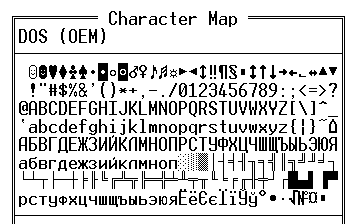
\includegraphics[width=5cm,height=3.128cm]{ideas/03_1_encodings/dos.png}&
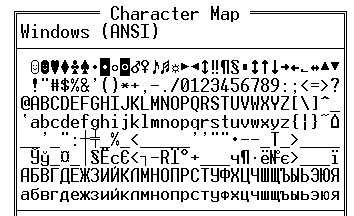
\includegraphics[width=5cm,height=3.128cm]{ideas/03_1_encodings/win.png}&
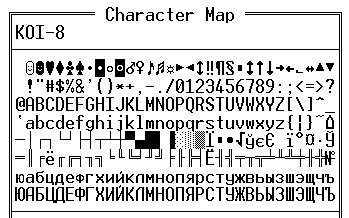
\includegraphics[width=5cm,height=3.128cm]{ideas/03_1_encodings/koi.png}\\
DOS (cp866)&Windows-1251&KOI8-R
\end{tabular}

Кодировки (первая строка "--- символы номер 0.\,.31, вторая "--- 32.\,.63 и т.д.). Получено просто 
с плагина Character Map к Far. Во второй половине таблицы в DOS корректно показаны все символы, в 
остальных таблицах "--- в основном только русские буквы, остальные символы могут быть неправильные. 
Зацените порядок русских букв в KOI8-R.

}

\vspace{0.2cm}

\hrule
\end{center}

Но со временем стало ясно, что 8 бит для представления текстов мало. Поэтому была изобретена 
\textit{кодировка Unicode}. В отличие от всех остальных распространённых сейчас кодировок, она не подразумевает 
использования 8 бит на символ.  Наиболее распространены, видимо, три варианта кодировки Unicode: 
\begin{ulist}
\item UTF-8, в которой на наиболее часто используемые символы (а именно, первую половину таблицы ASCII) 
используется один байт (8 бит, первый из которых 0), на некоторые символы (в т.ч. русские) "--- два байта (при этом, 
естественно, так, чтобы нельзя было перепутать с однобайтовыми символами "--- первый бит первого 
байта обязательно 1), а на некоторые "--- три или четыре (всегда по первым битам первого байта можно 
различить, какой из этих четырёх случаев имеет место). 
\item UTF-16: в ней часть символов занимает 2 байта, а часть "--- четыре. Я ни разу не помню, чтобы 
встречал эти четырехбайтовые символы, поэтому в первом приближении можно пренебречь их 
существованием и считать, что каждый символ UTF-16 занимает два байта.
\item UTF-32: все символы кодируются 4 байтами. Я лично сталкивался с этой кодировкой очень редко.
\end{ulist}
Кодировки Unicode сейчас весьма распространены (и вообще, есть люди, которые считают, что использовать
где-либо что-либо кроме Unicode нельзя, но я с ними до конца не соглашусь). Ещё замечу, что во всех 
этих кодировках возникает так называемая проблема 
byte endianness "--- проблема порядка байт: если на символ требуется больше одного байта, то какой 
из них писать первым, а какой вторым. Иногда пишут одним способом, иногда другим (на самом деле это 
проблема не только кодировки, но и вообще представления чисел).\footnote{\textit{Термины big-endian и little-endian первоначально не имели отношения к информатике. 
В сатирическом произведении Джонатана Свифта "<Путешествия Гулливера"> описываются вымышленные 
государства Лилипутия и Блефуску, в течение многих лет ведущие между собой войны из-за разногласия 
по поводу того, с какого конца следует разбивать варёные яйца. Тех, кто считает, что их нужно 
разбивать с тупого конца, в произведении называют "<Big-endians"> ("<тупоконечники">).} "--- 
\texttt{http://ru.wikipedia.org/wiki/Порядок\_байтов}}

И финальные замечания: если вы видите, что какой-то текст, который, как вы думали, должен быть 
нормальным русским текстом, выглядит набором странных символов, то, скорее всего, вы смотрите его в 
неправильной кодировке. Как правило, правильная кодировка "--- это одна из перечисленных выше. Если 
вы столкнулись с этой проблемой, просматривая сайт или электронную почту, то, как правило, это не 
составляет проблемы: большинство браузеров и почтовых программ позволяют вручную указать кодировку, 
в которой следует просматривать текст (т.е. они перед выводом на экран перекодируют текст из 
указанной кодировки). Если же это текстовый файл, то: Far 1.x благополучно умеет показывать кодировки 
Windows, DOS, а, если его подучить, то и KOI8-R (смотрите каталог \verb|Far\Addons\Tables\Cyrillic| при
желании). Unicode он может только показывать UTF-16, поэтому, что делать с Unicode, если его надо 
вручную редактировать или просматривать UTF-8 или UTF-32, однозначно посоветовать не могу. Можно 
открыть файл в браузере и вручную попросить нужную кодировку.

Наконец, приведу результаты просмотра текста `\texttt{Russian text Русский текст}', написанного 
изначально в разных кодировках, в кодировке DOS (т.е. изначальный текст я написал в разных 
кодировках, а потом стал просматривать в DOS):

\begin{center}
\hrule

\vspace{0.2cm}
\noindent\begin{tabular}{c|c|c}

\includegraphics[width=5cm,height=0.4cm]{ideas/03_1_encodings/rustext_dos.png}&
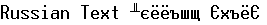
\includegraphics[width=5cm,height=0.4cm]{ideas/03_1_encodings/rustext_win.png}&

\includegraphics[width=5cm,height=0.4cm]{ideas/03_1_encodings/rustext_koi.png}\\
DOS&Windows&KOI8-R
\end{tabular}

\vspace{0.2cm}
\hrule
\vspace{0.2cm}

\noindent\begin{tabular}{c|c}
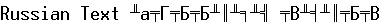
\includegraphics[width=7cm,height=0.4cm]{ideas/03_1_encodings/rustext_utf8.png}&

\includegraphics[width=9cm,height=0.4cm]{ideas/03_1_encodings/rustext_utf16.png}\\
UTF-8&UTF-16
\end{tabular}
\vspace{0.2cm}
\hrule
\end{center}

(Разные пропорции у разных символов "--- это ничего не значит, мне просто лень было подбривать 
размеры при вставке картинок в текст.) Конечно, текст, изначально написанные в кодировке DOS, 
нормально вполне в этой кодировке и просматривается; особых комментариев по тексту, изначально 
написанному в кодировках Windows и KOI8-R, я не придумал, но обратите внимание на следующие 
особенности Unicode-кодировок:


\begin{ulist}
\item UTF-8.  Обратите внимание, что английский текст (и все три пробела!) получился вполне нормальным, и только русский 
текст испортился. Обратите также внимание на некоторую довольно заметную двухбайтную периодичность 
в русском тексте
(т.е. на то, что чётные байты довольно сильно отличаются от нечётных: в чётных байтах встречаются 
то буквы, то символы псевдографики, а в нечётных "--- только два разных символа псевдографики).
Это общий признак кодировки UTF-8: если вы видите, что все английские буквы, 
цифры, знаки препинания и т.п. выглядят нормально, а вот там, где должны быть русские буквы, 
написана какая-то чушь с явной двухбайтовой периодичностью, то скорее всего, вы просматриваете 
кодировку UTF-8. Для примера картинка: отрывок из xml-файла, записанного в кодировке UTF-8 и 
просмотренного, на этот раз, в кодировке Windows. Все, кроме русских букв, как будто в однобайтовой 
кодировке, а в русских буквах явно видна периодичность в два байта. Обилие подчерков объясняется 
тем, что этим кодам в Windows-кодировке соответствуют одинаковые изображения (т.е. что в 
Windows-кодировке на этом месте не находятся никакие толковые символы типа русских букв и потому
этим символам не стали придумывать никаких умных картинок; та же причина, что и в обилии подчерков в
приведённой выше таблице символов для кодировки Windows).
\begin{center}
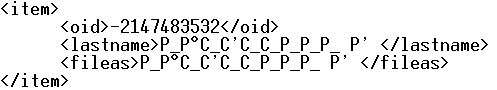
\includegraphics[width=8cm,height=1.44cm]{ideas/03_1_encodings/utf8_contact.png}
\end{center}

\item UTF-16. Обратите внимание, что на этот раз \textit{все} символы занимают по два байта. И 
английские, и русские буквы, и пробелы занимают два байта; при этом первый байт у английских букв и 
пробелов "--- символ номер ноль (который в этом шрифте имеет такую же картинку, что и пробел, и 
потому выглядит как пробел), а второй байт как раз и есть соответствующий символ (английская буква 
либо символ 32 для пробела). Первый байт у русских букв, как вы можете видеть из таблиц кодировок 
выше, есть символ номер 4, ромбик. Этот ромбик на самом деле является характерным признаком 
русского текста, написанного в кодировке UTF-16 и просматриваемого в однобайтовой кодировке (что 
DOS, что Windows), а "<разрежённые"> английские буквы и цифры (на самом деле, ещё раз, между ними 
не пробелы, а символы номер 0) "--- характерным признаком английского текста в кодировке Unicode. 
Ещё раз подчёркиваю, что, т.""к. вы, скорее всего, не будете сталкиваться с четырехбайтовыми 
символами в UTF-16, то можно приближённо считать, что UTF-16 "--- абсолютно двухбайтовая кодировка.
\end{ulist}

\note{Почему я привожу все отрывки здесь в виде картинок. Потому что в \TeX{}е используется на 
самом деле своя кодировка; при чтении входного файла он осуществляет перекодировку из входной 
кодировки в свою, при этом часть символов, естественно, теряется. Поэтому, чтобы донести до вас по 
возможности полное многообразие символов разных кодировок, я их вставляю картинками.}
% Исходный LaTeX-код (c) Пётр Калинин
% Код распространяется по лицензии GNU GPL (!)

\lheader{\texttt{'A' xor ' '='a'}}
Ещё одно замечание, имеющее непосредственное отношение к кодировкам, но не к основным идеям 
предыдущего параграфа. Обратите внимание, как расположены английские маленькие и заглавные буквы в 
таблицах кодировок, приведённых в предыдущем параграфе. Они расположены друг под другом. Этот 
обозначает, во"=первых, что их коды отличаются на 32, но ещё и, во"=вторых, что у всех заглавных 
букв в разряде, соответствующем степени $2^5=32$, в двоичной записи кода стоит 0, а у маленьких "--- 1. Учитывая,
что 32 "--- это код пробела, это обозначает, что \texttt{'A' xor ' '='a'} (на самом деле здесь, 
конечно, имеются ввиду коды букв, т.е. \verb|ord('A') xor ord(' ')=ord('a')|; паскаль вам ругнётся 
на предыдущей строчек. Если вы не понимаете, что значит тут операция \verb|xor|, то посмотрите один 
из далее идущих параграфов). Это замечание, конечно, позволяет очень быстро инвертировать регистр у 
английского текста, но все равно не даёт широких возможностей для практического применения: даже 
для того, чтобы инвертировать регистр у текста, который может содержать, помимо английских букв, 
ещё и другие символы, надо каждый символ проверять, является ли он английской буквой, что сводит на 
нет всю красоту инвертации регистра таким способом; аналогичные проблемы будут, если надо, 
например, перевести весь текст в верхний регистр.

\note{Если вам надо перевести текст в верхний регистр, то лучше воспользуйтесь встроенными функциями,
либо просто прибавляйте/вычитайте 32; тем не менее имхо сам факт красив.}


\header{Замечания о языке программирования}
Буду о паскале: Free Pascal и Delphi. Про Borland Pascal говорить ничего не буду, это уже совсем 
устаревшая IDE.

Не забывайте про комбинацию клафиш Ctrl-F1, т.е. не забывайте, что многое можно (либо 
правду, либо полуправду, но все равно идеи поймете) посмотреть в справке. Там, может быть, все 
будет не очень хорошо объяснено, но вы поймете и додумаете сами.

% Исходный LaTeX-код (c) Пётр Калинин
% Код распространяется по лицензии GNU GPL (!)

\lheader{Нетривиальные типы данных в паскале}

\textbf{Вещественные типы.} Как известно, в паскале есть 4 "<настоящих"> вещественных типа: 
real, single, double и extended (про comp разговор будет ниже). Из них последние три "--- 
стандартные типы, они поддерживаются математическим сопроцессором, который, насколько я понимаю, 
давно встроен во все современные  процессоры. А первый (real) в Borland Pascal обрабатывался 
полностью программно, из процессорных функций используя, 
видимо, только работу с целыми числами; в современных версиях это как правило или single или 
double, в зависимости от настроек (а, возможно, при определенных настройках это может быть и старый странный тип).  

Как итог, в других языках программирования есть типы, полностью совпадающие 
по структуре с signle и double (float и long float в C/C++, насколько я понимаю), и могут быть 
типы, полностью совпадающие с extended (типа long long float в некоторых компиляторах C/C++). 
Это, правда, нам будет фактически не  
важно, оно лишь приводит к тому, что, передавая, например, число типа single напрямую как оно записано в 
памяти "--- четырьмя байтами "--- в другую программу, вы без проблем сможете работать с ним там, 
даже если другая программа написана на другом языке, а вот с real не все так просто, надо понимать, какой именно это тип , "--- но такая 
необходимость в олимпиадных задачах возникает очень редко.
Аналогично, \texttt{file of single} (см. ниже) можно читать программой, написанной на любом (ну... 
почти любом "--- ещё бывают проблемы с порядком байт) языке программирования, а с \texttt{file of 
real} все сложнее.

Но все равно даже сам факт того, что real это либо single, либо double, либо что-то еще, делает тип real некоторым "<искусственным 
включением"> в системы типов. Это неудивительно: насколько я понимаю, во времена создания паскаля 
далеко не все компьютеры оснащались сопроцессором (да и, возможно, не было общепринятых стандартов 
хранения вещественных чисел в памяти), и потому был изобретён новый тип, чтобы можно было работать 
с вещественными числами и без сопроцессора. В современных же условиях нет необходимости так 
хитрить, и потому тип real фактически не нужен, поэтому его и приравняли к single/double. Поэтому 
фактически \textbf{никогда} не следует использовать в своих программах этот тип, пользуйтесь лучше single, double или extended. 

Какой же из трёх оставшихся типов использовать? Конечно, все зависит от задачи. Операции с single 
выполняются довольно быстро (но тем не менее, конечно, много дольше, чем операции с целыми 
числами), но, как правило, точности single не хватает в олимпиадных задачах (хотя в неолимпиадных 
вполне может хватать). Double обычно 
обеспечивает достаточную точность, но работает дольше, чем single. Extended обеспечивает ещё 
б\'{о}льшую точность, но ценой несоразмерного увеличения времени обработки. (Ну и, конечно, типы 
расходуют разное число байт: single 4, double 8, extended 10.) Тем не менее я всегда 
использовал где можно extended, и только если начинались проблемы с памятью или временем, переходил 
на double или в крайнем случае single. ИМХО, как правило, в олимпиадных задачах, где требуется 
вещественная арифметика, обычно время и память не столь критичны, чтобы надо было от extended 
уходить к другим типам.

Кстати, не забываем, что при работе с вещественными числами нельзя писать \verb|if a=0| и т.п., а надо работать с \verb|eps|.

\textbf{Нетривиальные целочисленные типы.} Пожалуй, ограничусь просто перечислением.
\begin{ulist}
\item \texttt{integer}. Казалось бы, ничего особенного, но в FP он занимает 2 или 4 байта в 
зависимости от настроек, и хранит соответствующий диапазон чисел. Советую в FP всегда писать 
\verb|{$mode delphi}| (см. ниже), и не иметь проблем. Двухбайтный тип, 
аналогичный BP'шному integer, называется smallint (а есть ещё и однобайтный shortint, такой же, как 
и в BP). 
\item \texttt{cardinal}, он же \texttt{longword}\footnote{Тут, похоже, есть какая"=то очень тонкая 
разница, связанная с поведение на разных платформах и ОС, но я её не знаю}. Это беззнаковый 
32-битный тип (т.е. как word относится к integer, так cardinal относится к longint). 
Соответственно, позволяет хранить числа от 0 до $2^{32}-1\approx 4\,000\,000\,000$.
\item \texttt{int64}. Знаковый (т.е. может хранить отрицательные числа) 64-битный тип. 
Хранит числа от $\approx -2^{63}$ до $\approx 2^{63}$ (пишу 
$\approx$, т.к. там где"=то граница отличается на единицу от степени двойки, даже понятно, где). 
\item \texttt{comp}. Аналогично int64 знаковый 64-битный тип. Но, в отличие от int64, он, видимо, 
поддерживается \textit{не} самим процессором, а сопроцессором (могу и ошибаться!). Поэтому есть ряд 
особенностей: во"=первых, comp был доступен даже в BP, во"=вторых, 
компилятор считает его вещественным типом со всеми вытекающими отсюда последствиями. В т.ч. его 
нельзя напрямую присваивать переменным целого типа, надо делать \texttt{round} и т.п.; с ним не 
работает \texttt{mod} и \texttt{div}, зато работает \texttt{/}, которое "--- внимание! "--- 
округляет результат по правилу round: 5/3=2, если считать в comp; при выводе в файл или на экран 
надо писать \verb|:0:0|, иначе будет вывод в виде с плавающей точкой (\verb|2.36348e5| типа того); 
кроме того, при выводе могут произойти глюки: существует небольшое количество значений comp, 
которые даже с \verb|:0:0| выводятся с ошибкой в паре последних знаков (хотя в памяти хранится 
точное значение!), поэтому с ним надо быть всегда осторожным. Т.е. comp выполняет все вычисления в 
пределах 64-битных целых значений абсолютно точно (как и любой целочисленный тип в пределах своей 
области значений), но есть приколы, которые надо понимать. Поэтому не используйте comp, используйте 
int64!
\end{ulist}
\lheader{���� ���������}
���� ��������� ��������� ������ �� ��������� ��������� � �⤥���� �����. �� ���� 
��ଫ����� � ���� ��ப� \verb|{$...}|, �.�. ��� ����� �������਩, �� ��稭��騩�� � ᨬ���� 
\verb|$|. ����設�⢮ ���祩 ����� ���� ���� ��� ����祭�, ��� �몫�祭�, �, ᮮ⢥��⢥���, 
�������, ���ਬ�� \verb|{$R+,Q+,S+,I+,B-}|; ������� ���� ����� ��㣮� �ଠ�.

������� ����� ᮮ⢥����� ������� ���� � ����ன��� �����窨 (IDE) ��᪠��; ⥬ �� �����, 
����, 㪠����� � 䠩�� � �ணࠬ���, ����� ����� ��᮪�� �ਮ���. � ����, �� � ��砫� �ணࠬ�� ����������� 
���� ������� � ����, ����� ��� ����� (� ����� ��।� \verb|r|, \verb|q|, \verb|s|, \verb|i|, 
\verb|mode| � �������� \verb|o|), �⮡� ���� 㢥७�묨, �� ��� �ணࠬ��  
�㤥� � ��� �������஢����� � ⥬� �� ���砬�, �� � � ���.

���祩 �����쭮 �����, � ������ ���� �, ����� ��� ��室���� ������ ��� �� �ࠩ��� ��� ��������, �� ��� ������.

\textbf{���� }\verb|$I|, \verb|$R|, \verb|$Q|, \verb|$S| �������/�몫���� ࠧ���� �஢�ન:
\begin{ulist}
\item \verb|$I| "--- �஢��� �� �⥭�� ������ �� 䠩��. �᫨ �� ������ (\verb|{$I+}|), � �� 
��� ����� �᫮ �� 䠩��, � ⠬ ����ᠭ� �㪢�, � ��� �ணࠬ�� �뫥�� � Runtime Error. 
�᫨ ���� �몫�祭, � �訡�� �� �ந������, ��, ����筮, ��⠥��� �����஥, ᪮॥ �ᥣ�, 
���ࠢ��쭮�, �᫮.
\item \verb|$R| "--- �஢��� �� ᮮ⢥��⢨� ࠡ��� � ������� ࠧ��ࠬ �뤥������ �����. � 
������, �஢������ ��९������� ���ᨢ� (��୮ ��, �� �� ���饭�� � �������� ���ᨢ� �� �� 
��室�� �� ��� �࠭���), � �� ����� ���祭�� � ������ ��६����� �ந�室�� �஢�ઠ, ������� �� 
���祭�� ��६����� � ������, �뤥������ ��� ��� (�� ��⠥��� �� �� ���祭�� 1000 ��࠭��� � 
��६����� ⨯� byte). �᫨ ���� ������, � �� �����㦥��� �訡�� �ந������ Runtime Error 
(�����⭮, Range Check Error "--- RE 201),  � �ணࠬ�� ��� �� ������� ࠡ���. �᫨ �몫�祭, � 
�ந������ �������⭮ ��. � ��⭮��, �᫨ �� ��⠫��� ������� ����� �� �।��� ���ᨢ�, � ���� 
�몫�祭, � ������ �� ࠢ�� �ந������. �� �⮬ �㤥� ������ � ���祭��, ���஥ ⠬ ������, � 
⠬ ����� ������ ���祭�� ��㣮� ��६����� ��� ���� �ᯮ��塞� ��� ��襩 �ணࠬ��. � १���� 
���쭥�襥 ��������� ��襩 �ணࠬ�� �।᪠���� ���� ����������, ��� ����� ������ ���������� 
���, � ����� ᫮������ ����⫥���, �� �ணࠬ�� <<�室�� � 㬠>>. ���⮬�, �᫨ �ணࠬ�� ������ 
��"=� ��࠭���, �஢����, �� �易�� �� �� � ��९�������� ���ᨢ� "--- ���� ������ ���� 
\verb|$R|, �, ��������, �� ������, � 祬 ����.
\item \verb|$Q| "--- �஢��� �� ��९������� �� �஬������� ���᫥���� ($+$, $-$, $*$, abs � 
�.�., �� \textit{��} inc � dec). �᫨ � ��� � �ணࠬ�� ����ᠭ� �����஥ ᫮���� ��䬥��᪮� 
��ࠦ���� � 楫묨 �᫠��, � �� �஬������� ���᫥���� ����� �ந���� ��९�������: 
१���� �஬����筮�� ���᫥��� ����� �� ������ � ������, � ���ன �� ���᫥��� 
�ந��������. �᫨ ���� \verb|$Q| ������, � � ⠪�� ��砥 ������ Runtime Error (�����⭮, 
Arifmetic Overflow "--- RE 215), � �ணࠬ�� ��� �� ���������. �᫨ �몫�祭, �, ᪮॥ �ᥣ�, 
��������騥 ���� ���� ���� ���襭� � ���᫥��� ���� �த������ � ����祭�� ���ࠢ���� 
���祭���. � ��⭮��, ��� � १���� � �⢥� ����砥��� ����⥫쭮� �᫮, ���� �᫨ ��� 
⠬ ��⥬���᪨ �� ����� ���������.
\item \verb|$S| "--- �஢��� �� ��९������� �⥪�. �᫨ ���� ������, � �� ������ �맮�� 
�㭪樨 �㤥� �஢������, �����筮 �� �⥪� �, �᫨ �������筮, � �㤥� Runtime Error (Stack 
Overflow "--- RE~202), � �ணࠬ�� ��� �� ���������. �᫨ ���� �몫�祭, � �஢�ન �� �������� 
�, �������筮 ����� \verb|$R|, �ணࠬ�� ����� ���񧭮 <<ᮩ� � 㬠>>.
\end{ulist}
���⮨��⢠ ����祭�� ��� ������ ���祩 ����� � ⮬, �� �� �ࠧ� 㢨��� �訡��, ������ � 
��砥 �몫�祭��� ���祩 �뫮 �� �祭� ᫮��� �᪠��. 

� ������, �᫨ ���� �� ��� �訡�� ������ �� �������� �����, �:

����� ⮦� ����� ����ந�� ⠪, �⮡� �� �訡�� 
��� �����뢠�� ��ப� (��-�����, ��� �⮣� ���� ��������� unit SysUtils), � ��᫥ �⮣� �� 
����᪥ �ணࠬ�� ��� �㤥� ��������, �� ����� ��ப� � ��� �訡��.

� FP �⮡� 㢨���� ��ப�, �� ���ன �訡��, ���� ��। ����᪮� �ணࠬ�� ���� � ०�� �⫠���, 
�.�. ������ F8, � ⮫쪮 ��᫥ �⮣� Ctrl-F9.
                                             
����� ⮣�, �᫨ �� ���� �� ����� 㧭���, �� ����� ��ப� �訡�� (���ਬ��, �᫨ �訡�� �ந��諠 �� 
���஢���� ����� �� �ࢥ� ���), �� �� ࠢ�� 㧭���, �� �ந��諠 ������ ⠪�� �訡�� (��� 
ᮮ��� RE, � �� WA), � �� �㤥� �����, �� ���� �᪠�� ��-� ��������. �������, �᫨ ���� 
�몫�祭�, � ��᫥ �訡�� �ணࠬ�� ᯮ����� ᥡ� �㤥� ࠡ���� �����, ��, ᪮॥ �ᥣ�, 㦥 � 
���ࠢ���묨 ����묨. � �⮣� �஡���� �ᯫ��� ᮢᥬ � ��㣮� ���� ��� � ��㣮� ����稨, � �� 
�㤥� �᪠�� �訡�� ᮢᥬ �� ⠬ ��� �㤥� �᪠�� ᮢᥬ �� �� �訡��. ���ਬ��, ����� 
���������, �� � ��室��� 䠩� �뢥���� ����⥫쭮� �᫮, �� ⮬, �� ������ ���� 
������⥫쭮�, ���, ���ਬ��, �� �㤥� ������ ������, ��祬� �� ��।��� ��ப� ��������� 
���祭�� ��६����� $i$, �� ⮬, �� ��� ����� � �⮩ ��ப� �� 㯮��������, ��� �� �뢮�� 
�⢥� � 䠩� ��� ������� File not open for output, �� ⮬, �� � ��� �� ��ଠ�쭮 � ࠡ�⮩ � 
䠩����, ��� �ணࠬ�� �㤥� ࠡ���� ����� � ��横�������� � �.�. � �.�. 

������⪮� �� ���: ��"=�����, ��� �ணࠬ�� �㤥� ����ଠ������, ��⮬ ��।�� �� �㤥� �祭� 
����⭮; ��"=�����, �᫨ ���� �ந��諠 ���� �� ��� �訡��, ���� (�祭� �����쪠�) ����⭮��� 
⮣�, �� � �몫�祭�묨 ���砬� �� ࠢ�� ��� �ணࠬ�� �뢥��� ���� �⢥� � ��� �㤥� 
�ன���.

� ��饬, ���� ����� ࠧ �㬠�� �������, ���� �� ��� ������� ��� �몫���� �� ���� (�� � �� 
��砥 ���� �� ��� � ������� � �ணࠬ��, ��� � �몫����! �⮡� �� ������� �� ⮣�, ����� 
����ன�� �� 㬮�砭�� � ��� ��� � ��襣� ���������). ����, �� �६� ࠧࠡ�⪨ �ணࠬ�� ���� 
\textsc{��易⥫쭮} ������ ���� ����祭�, �⮡� ��� ���� �뫮 �⫠������� �訡�� �� ���� �� 
����. ����� �� �� ᤠ�� �ணࠬ��, � ��� ���� �㬠��.

� \textit{誮����} ���������� ����筮 �몫���� ���� ��। ᤠ祩 �ணࠬ�� �� 
�஢���: ������� ���� ��� ⠬ 㦥 �� �������, ��� ����� 1. ���ମ���� �ணࠬ�� � 2. ����� 
��砩�� ��������, �� � �몫�祭�묨 ���砬� �ணࠬ�� �ࠢ��쭮 �ன��� ���, �� ���஬ �� 
�������� ����� ��� 
�뫥⥫� �� � RE. � ���������� �� \textit{⨯� ACM}, ��� �� ����� ������ १����� ���஢���� ��襩 
�ணࠬ�� � �������஢��� �� ��� ��ࠢ����� �ணࠬ��, ����� ����� ��� ᤠ���� �ணࠬ�� � � 
������묨 �஢�ઠ��: ᮮ�饭��, �� � ��襩 �ணࠬ�� RE, ��� ������� ������� �����, 祬 WA.

����, ���� �訡��: �᫨ ��� �ணࠬ�� �뫥⥫� � ����� �� ��� Runtime Error, � �������: 
������ ���� �몫�稬 ᮮ⢥�����騩 ����, � �訡�� ��祧���... ���! �ࠡ��뢠��� ������ �� ��� 
���祩 㪠�뢠�� �� ����稥 ���񧭮� �訡�� � ����. �⪫��� ����, �� ���� 㡨ࠥ� �����饭�� � 
���, ᠬ� �訡�� �������. �᫨ �ந��諠 ⠪�� �訡��, ���� ࠧ�������, � 祬 ���� � ��ࠢ���� 
�᭮���� ��� �ணࠬ��!

��᪮�쪮 � ����, � C/C++ ��� ��饯ਭ���� ᯮᮡ�� ����஫� �������� �訡�� (���⮬�, � ��⭮��, 
�஡���� � ��९�������� ����� ������ �� �����쭮 ����� � ��㤭�㫮����� �訡�� � �ணࠬ�� �� 
C/C++). ����� ��� �� �� ���� ����.

\textbf{����} \verb|$B| ����� �� ��ࠡ��� ��ࠦ���� ⨯�
\begin{codesampleo}\begin{verbatim}
if (n>0)and(f(n)>0) then
\end{verbatim}\end{codesampleo}
�.�. ����� � ��� � if ��� ��� ����� �᫮���, �易���� �����஬ or ��� and. � ⠪�� ��砥 ��᫥ 
���᫥��� ��ࢮ�� �᫮��� ����� ���������, �� �� ���祭�� ��ண� �᫮��� ��祣� �� ������ 
(���ਬ��, � �ਢ��񭭮� �ਬ��: �᫨ $n\leq0$, � �஢����� $f(n)$ ����祬: � �� ��砥 if �� 
�믮������). �᫨ ���� \verb|$B| \textit{�몫�祭}, � � �������� ����� ��஥ �᫮��� 
�஢������� �� �㤥�, ���� �㤥�. ����� ����������, �� ���� �� ���� �������� ��䥪�, �஬� 
�먣���/�ந���� �� �६���, �� �� ᠬ�� ���� �� �� ⠪. ��஥ �᫮��� ����� ����� �����-����� 
������ ��䥪�� � ⮣�� �ணࠬ�� �㤥� ࠡ���� ��"=ࠧ���� � ����ᨬ��� �� ���� \verb|$B|; 
���ਬ��, �᫨, ��� � �ਬ�� ���, � ��� �� ����� ᪮���� ���� �맮� �㭪樨, � �� $n\leq0$ ��� 
�㤥� ��� �� �㤥� �맢��� � ����ᨬ��� �� ���� \verb|$B| "--- � � �㭪�� ����� ������ �祭� 
����� ��. ����� ���������� ��࠭��, �� � ����設�⢥ ��砥� ��� �㦭� ��� ࠧ ���������, 
ᮮ⢥�����饥 �⪫��񭭮�� �����, \verb|$B-| "--- ����⢨⥫쭮, ⠪�� if, ��� ���, ��, 
��������, ����ᠫ� ��⮬�, �� ��� �㭪�� ���� ��ࠡ��뢠�� ���祭�� $n\leq0$ "--- �����, �� 
����⢨⥫쭮 �� ���� ��뢠�� � ⠪�� ��砥. ��� ��� �ਬ��, ����� ���� \verb|$B| �����:
\begin{codesample}\begin{verbatim}
if (n>0)and(n<maxn)and(a[n]=k) then
if (x>=0)and(sqrt(x)<y) then
\end{verbatim}\end{codesample}
����� ���㬠��, ����� ��� ��������� �஡����, �᫨ ��� ��� �㤥� ᪮�����஢�� � \verb|$B+|.

\textbf{����} \verb|$A| ����� �� ⠪ ���뢠���� <<��ࠢ�������>> (alignment). ���६���� 
�����奬� ��� ⠪ ���஥��, �� ����� � ��� ���� 
�ந�室�� ����॥ ��� ���������, � ����ᨬ��� �� ⮣�, ��稭����� �� ��� � ��⭮�� ��� � 
����⭮�� ����. �������筮 �६� ����㯠 � ���થ ���� ����� ������� �� ���⪠ �� ������� �� 4 
����� ��ࢮ�� ���� ���ન � �.�. ���⮬� ��� ��⨬���樨 �६��� ����㯠 ���������� ����� 
�믮����� "<��ࠢ�������"> ������, �.�. ������ ⠪, �⮡� �� ��६���� ��稭����� � ���ᮢ, 
����� 4 (��� 2, ��� 8, ��� 16, ��� ࠧ���� ᠬ�� ��६�����, � ����ᨬ��� �� ����஥�), �� ����室����� 
��⠢��� ���ᯮ��㥬�� ����࠭�⢮ (�����) ����� �ᥤ���� ��६���묨.
�������筮 ����� ��ࠢ�������� �� ���� � record'�� � �.�. �� �� ��ࠢ������� � ����� ���� 
\verb|$A|. �᫨ ���� �몫�祭, � �������� ��ࠢ������� �� �믮������, ��६���� � ���� � 
record'�� ���� �����, �� �६� ����㯠 � ��� ����砥��� �����. �᫨ ���� ������, � �ந�室�� 
�����஥ ��ࠢ������� �� 㬮�砭��, �. ���஡��� � �ࠢ��. ����� ⠪�� � 㪠���� �ॡ㥬�� 
��ࠢ�������, 㪠��� �����⭮� �᫮ (\verb|{$A8}| � �.�.), ���஡��� ⮦� �. � �ࠢ��.

\textbf{����} \verb|$O| ����砥� ��� �⪫�砥� ࠧ���� ��⨬���樨, ����� ����� �ਬ����� ���������. � ०��� \verb|{$o+}| �ணࠬ�� ࠡ�⠥� ����॥, ��ன ���⨬� ����॥, �� �⫠������ �� ������� �殮���.

\textbf{����} \verb|$mode| �� Free Pascal ��⠭�������� ०�� ࠡ��� ���������, ����� ࠧ�� ��� ��ࠬ����:
���ਬ��, ��������� ⨯� \verb|integer|, ⨯� \verb|string|, ����稥 ��६����� \verb|result| � �㭪��� � �.�. �ᥣ�� ४������� ����� \verb|{$mode delphi}|, �᫨ �� ⮫쪮 㢥७�� �� ��������, ��祬� �⮨� ����� ���-����� ��. ����� \verb|delphi| ������ \verb|integer| 4-���⮢�, ������ \verb|string| �ந����쭮� ����� (� �� ⮫쪮 �� 256 ᨬ�����), �������� �ᯮ�짮���� ��६����� \verb|result| � �㭪���, � �.�.

����� ���ᠭ�� ࠧ����� ���祩 ���������.

��� ᪠�� �� ⠪ ���뢠��� "<conditional defines">. � �ணࠬ�� ����� �ᯮ�짮���� ⠪�� ���� 
��������� \verb|$define|, \verb|$undef| � \verb|$ifdef|/\verb|$else|/\verb|$endif|. ���� ��� � 
祬: �� �⥭�� ��室���� ⥪�� ��襩 �ணࠬ�� � ����� ������ � ��������� ���� ������� 
�����, �᫮��� ������, "<��権 �᫮���� �������樨">. ����� "<����"> "--- �� ���� �ந����쭠� 
��ப� �� ��⨭᪨� �㪢. �������� ��㡮���� ��᫠ � ��� ����砫쭮 ���, �� �ᯮ���� �� ��樨 
⠪, ��� ��� �㦭� �㤥�.

� ������, ���� \verb|$define| �������� �������� ���� � �⮬� ᯨ�� ��権: 
\verb|{$define optname}| �������� ���� \verb|optname| � �.�. ���� \verb|$undef| "--- 㤠���� 
���� �� ᯨ᪠ (�᫨ ��� ⠬ ����): \verb|{$undef optname}|. � ⥯��� �������: ���� 
\verb|$ifdef|/\verb|$else|/\verb|endif| ��������� �஢�����, ��।����� �� � ��� ���� ����: � 
������, �᫨ � ���� ���� ��᫥����⥫쭮��� 

\begin{center}
\verb|{$ifdef optname} some code {$else} other code {$endif}|
\end{center}
�, �᫨ ���� optname �室�� � ��� ᯨ᮪ � �������, ����� ��������� �⠥� ������� ifdef (� 
�⠥� �� 䠩�"=�ணࠬ�� ��ᨬ���쭮 �� ��砫� � �����),  � ��� ��᮪ ���� �㤥� ����� 
\textit{��᮫�⭮ ⠪�� �� ���}, ��� ��� �� ��� ���� ���� ��室���� ��� \verb|some code|,
���� "--- ��� ��� �� ��� ���� ��室���� ��� \verb|other code|. ����� else, ����筮, ����� ���� 
���饭�.

�ਬ���:

\begin{center}
\verb|{$ifdef check} {$r+,q+,s+,i+} {$else} {$r-,q-,i-,s-} {$endif}|
\end{center}
 "--- �᫨ ���� check "<����祭�">, � ����砥� �� �஢�ન, ���� �⪫�砥�. ���ਬ��, ����� 
������� � ��砫� �ணࠬ��

\begin{center}
\verb|{$define check} {$ifdef check} {$r+,q+,s+,i+} {$else} {$r-,q-,s-,i-} {$endif}|
\end{center}
 "--- � �� �஢�ન ���� ����祭�. �� ���� �ணࠬ��, ������ ��, � ��। ᤠ祩 �� �஢��� 
�������� \textit{���� �஡��} � ��� ���:

\begin{center}
\verb|{ $define check} {$ifdef check} {$r+,q+,s+,i+} {$else} {$r-,q-,s-,i-} {$endif}|
\end{center}
 "--- ��ப� \verb|$define check| �ॢ�頥��� � ����� �������਩ (� �� ��४⨢� ��������� :) 
) "--- � �� �஢�ન �⪫������.

��� �ਬ��:

\begin{center}
\verb|{$ifdef debug} writeln(output,i,' ',j,' ',a[i,j]);{$endif}|
\end{center}
�������� ��������� ��ࠧ�� �ࠢ���� �⫠���� �뢮���. 

��� �ਬ��:

\begin{center}
\begin{verbatim}
{$ifdef for}for i:=1 to 10 do{$endif}
  writeln('!');
\end{verbatim}
\end{center}
� ����ᨬ��� �� ���ﭨ� ��樨 �㤥� ���� 横�, ���� �����筠� �������.

���⮨��⢮ �⮣� � ⮬, �� ���� ��������/㡨�� �஡�� (��� �� ��㣮� ᨬ���) � ��砫� 
��४⨢� define, �� �ࠧ� ������� ��������� �ணࠬ��. (���ਬ��, � ��� � �ணࠬ�� ���� ��� ��� 
�⫠��筮�� �뢮��. �⮡� ��� ����, ����� ������ �㦭� ���������஢��� \textit{��} ��� ��ப�. 
�� �᫨ �⫠���� �뢮� ��ଫ�� ⠪, ��� � ������� ���, � �����筮 �������� � �ணࠬ�� ���� 
ᨬ���.)

��� ���� ���⮨��⢮: \textit{����砫쭮}, �� ��砫� �⥭�� �ணࠬ�� ��������஬, ᯨ᮪ ��権 �� 
��易⥫쭮 ����. �� ����� � BP � ���� Options---Compiler---Conditional Defines (� Delphi ���� 
���"=� ��������� �㭪�) ��।����� 
����砫�� ᯨ᮪ ��権, ����� �㤥� ����⢮���� �� �������樨 �� �।� �ணࠬ��஢���� 
\textit{� ⮫쪮 �� ���}; � ��� ��砫�� ᯨ᮪ �㤥� ��㣨�. ���ਬ��, � ���짮����� ᫥���騬 
��񬮬: � �⮬ �㭪� � ���� Options 㪠�뢠� check, � � ��砫� �ணࠬ�� ��ᠫ

\begin{center}
\verb|{$ifdef check} {$r+,q+,s+,i+} {$else} {$r-,q-,i-,s-} {$endif}|
\end{center}
"--- � � ���� �� �����窨 ����������� � ������묨 ���砬�, � � ��� "--- � �몫�祭�묨 :). 
�ࠢ��, � �⮬ ⮦� �뫨 ᢮� ��㤮��⢠\dots

�������筮, � ����ᨬ��� �� �।�, � ���ன ������������ ��� �ணࠬ��, ������� ��樨 ����� 
���� ��।����� ��࠭��. ���ਬ��, ���� ��樨, ����� ��������� ࠧ�����, ����������� ���� 
�ணࠬ�� ��� Windows ��� Linux, ��� ����� ������ ��������஬, ������ �ࢥ�� ������-�஢�ન 
��⠭�������� ����, �����뢠�騩, �� �ணࠬ�� ������������ �� �⮬ �ࢥ�, � �.�.

��� ࠧ �����ન���, �� �� �� ����� ⮫쪮 �� ���������. ���⮬�, ���ਬ��, ����� ⨯�

\begin{center}
\begin{verbatim}
for i:=1 to n do begin
  {$ifdef check}
  writeln('!');
  {$endif}
  {$define check}
end;
\end{verbatim}
\end{center}

� �����뢠��, �� �� ��ன � ����� ������ 横�� check �㤥� ��।�����, �����᫥���: 
��������� �⠥� �室��� 䠩� �� ���浪�, �� ����� �������� �� 横�� � �.�., � ���� �� ������ 
��� \verb|writeln('!')| � exe'譨�.

�, �������, ��� ࠧ. ����筮, �� �ᯮ���� �� ��, �᫨ �� �� �� ��������. ���砫� ������, 
��������, �஢����, �� �� �� �ࠢ��쭮 ��������, � ��⮬ ⮫쪮 �ᯮ����.


% Исходный LaTeX-код (c) Пётр Калинин
% Код распространяется по лицензии GNU GPL (!)

\lheader{Битовые операции} Всем известны логические операции and, or, xor, not. Они из двух 
boolean"=значений делают одно: $true \OR false = true$ и т.п.. Существуют аналогичные операции
для \textit{чисел}, которые выполняют соответствующие действия побитово. В паскале эти действия
записываются теми же операторами, что и логические. Таким образом, например, $3 \OR 5= 7$, так как
$3=\dots00011_2$, а $5=\dots00101_2$, поэтому, если про-or-ить побитово (т.е. столбиком, т.е. 
младший бит с младшим и т.д.), то 
получится $\dots00111_2=7$. Аналогично $3 \AND 5 = 1$ и $3 \XOR 5 = 6$ (xor "--- исключающее ИЛИ, 
т.е. равно 1, только если \textit{ровно} один бит из двух равен единице, или, что то же самое, если 
два бита различны).

С побитовым not немного хитрее: т.к. \textit{каждый} бит инвертируется, то результат зависит от 
того, сколько всего бит было в числе, т.е. от типа, в котором вы проводите вычисления. Например, в 
byte будет, видимо, $\NOT 5= 250$.

\task|Поэкспериментируйте с операцией not в других типах. В частности, верно ли, что в 
знаковых типах (shortint, integer, longint) not может давать отрицательные значения? Должен бы.|||||

Кроме этих операций, есть ещё две довольно полезных: shr и shl. Операция shr (shift-right) осуществляет 
сдвиг битовой записи "<вправо">\footnote{Кавычки потому, что не очень"=то ясно, где здесь право, а 
где лево :). Младший разряд "--- это правый или левый?} на указанное количество бит, при этом 
младшие биты отбрасываются (т.е. операция эквивалентна  
делению на степень двойки): $2=4 \SHR 1=8 \SHR 2=16\SHR 3=32\SHR 4$ (т.е. $32 \SHR 4$ "--- это 32 
сдвинуть на 4 бита вправо). Кроме того, $2=5\SHR 1=11\SHR 2=18\SHR 3=40\SHR 4$, и $5\SHR 4=0$, т.к. младшие биты 
отбрасываются. Операция shl сдвигает битовую запись влево, дополняя младшие разряды нулями (т.е. 
эквивалентно умножению на степень двойки). Старшие 
разряды, вылезающие за тип, видимо, отбрасываются. Результат, конечно же, зависит от типа. Пример: 
в любом типе $2\SHL 1=4$, $5\SHL 4=80$; если влезет в тип, то $1\SHL k=2^k$.

\task|Поэкспериментируйте с операцией shl в других типах. В частности, верно ли, что в 
знаковых типах (shortint, integer, longint) shl может давать отрицательные значения? Вроде действительно может давать.|||||

Огромное достоинство битовых операций состоит в том, что они выполняются \textit{очень} быстро (см.
также ниже, в параграфе про скорость операций). Например, делить на два с помощью shr~1 намного 
быстрее, чем с помощью div 2. Это, правда, не всегда важно "--- если операций деления на два у вас 
не так много, то сильно программу замена div~2 на shr~1 не ускорит, но иногда может помочь (см. также там же ниже). А вот возведение 
двойки в степень писать как $1\SHL k$ намного проще, чем циклом, и работать будет быстрее. Только 
ВНИМАНИЕ: стандартная ошибка "--- написать тут 2 вместо 1: например для деления на 2 написать 
shr~2 по аналогии с div~2 :) вместо верного shr~1, аналогично можно случайно написать $2\SHL k$ для 
возведения 2 в степень $k$. Это, конечно, приведёт к неправильному результату.

Битовые операции вы применяете, обычно, тогда, когда вам действительно надо что"=то сделать, 
связанное с битами. Например, число из $k$ единиц ($11\dots1_2$) можно получить как $1\SHL k-1$. 
Входит ли $k$"=я степень двойки в двоичное представление числа $n$ можно проверить так: $(n \SHR k) 
\AND 1=1$ или "--- второй способ "--- $n \AND (1 \SHL k)<>0$. В частности, проверить, чётно или нечётно число можно, 
посмотрев, чему равно $n \AND 1$, и т.п.

Обратите внимание, что я везде, где надо, ставлю скобки. Т.к. запомнить порядок действий здесь я не 
могу, то лучше для однозначности ставить скобки.

\task|Как быстро с помощью битовых операций вычислить максимальную степень двойки, на 
которую делится данное число? Ответ должен быть просто арифметическим выражением, без всяких циклов 
и т.п. и, например, для числа 40 давать ответ 8.
||Пусть нам дано число $N$. Посмотрите, чем $N-1$ отличается от $N$ в битовой записи.
||Пусть $N$ оканчивается на $k$ нулей, перед которыми идёт единица. Тогда ответ на наш вопрос будет $100\dots0_2$ "--- единица с $k$ нулями на конце. Как это вычислить? Заметим, что $N-1$ заканчивается на $k-1$ единицу, перед которыми идёт ноль (просто вычтите единицу из $N$ столбиком), т.е. отличается от $N$ ровно в $k+1$ последних битах. Тогда $N \XOR (N-1)$ будет равно $11\dots1_2$ "--- число, состоящее из $(k+1)$ единицы, "--- и $((N \XOR (N-1)) +1) \SHR 1$ даст то, что нам надо. Вообще, идея про-xor-ить $N$ и $N-1$ для выделения нулей на конце числа $N$ довольно часто встречается.
|

Ещё частое употребление "--- если вы числом $n$ кодируете последовательность нулей и единиц 
(закрашенных и незакрашенных клеток, используемых и не используемых объектов и т.п.), и вам надо 
что"=то с ней сделать (определить, закрашена ли та или иная клетка), то почти всегда подобные действия можно перевести на язык битовых операций.
\lheader{"<������"> ����"=�뢮�} �� �४�᭮ �����, ��� �������/�뢮���� ����� ��/� 䠩�, � 
���஬ ����� ����ᠭ�/������ ���� ����ᠭ� plain text, �.�. ���� ⥪�⮬, �����, �� �������, ����� 
������ 祫����: �� �ᯮ���� ⨯ text � ��, �� � ��� �易��. � १���� �� �᫠ � 䠩�� 
��������� � ���� ��᫥����⥫쭮�� �������� ��� � �.�. �� ����� ��������, �� �� ���쬠 
���������� ᯮᮡ �����/�뢮��: �� �ॡ�� �����쭮 ���ਢ���쭮� ��ࠡ�⪨ �� ��ॢ��� �᫠ �� 
⮣� ����, ��� ��� ����ᠭ � 䠩��, � �� ���, � ���஬ ��� �࠭���� � ����� �������� � 
�ᯮ������ �ணࠬ���, � �������; �஬� ⮣�, �᫠ � 䠩�� �������� ������� ����� ����, 祬 
����� �� (��� ����� ���祭�� ⨯� integer, ���ਬ��, ����� ���ॡ������� 5 ��� + ���� + �஡��, � � 
�६� ��� �� ᠬ�� ���� ��� ����஢���� ���祭�� integer �����筮 ���� ����). �᭮���� 
���⮨��⢮ ⠪��� �ଠ� ��⮨� � ⮬, �� ��� ����� ��� �ᮡ�� ࠧ�㬨� ������ 祫����.

�� �뢠� ��砨, ����� ����� �����/�뢮�� � ���������� ���� �⠭������ ����� �����, 祬 
"<�⠡��쭮���"> �뢮��. ��� �⮣� ������� ����������� �����뢠�� ����� � 䠩� �����।�⢥��� 
⠪, ��� ��� �࠭���� � �����: �᫨ � ����� �᫮ 28454 ($={\rm6F26}_{16}$) ⨯� integer �������� 2
����, � ����� ����ᠭ� ���祭�� 111 ($={\rm6F}_{16}$) � 38 ($=26_{16}$) (� �筮���� �� ���浪� 
����, �. ����), � � � 䠩�� �� �� �᫮ ������ ��� ����, � ����� ���� ����ᠭ� � �� 
���祭�� 6F � 26. �����, � ����� ����� ����ᠭ� ⠪�� ᯮᮡ��, ��� ���뢠�� "<�����묨"> (� 
����� 䠩�� � �⮬ ��᫥ "--- "<⥪�⮢묨">),  
ᮮ⢥��⢥��� ⠪�� ᯮᮡ �����/�뢮�� ����� ���뢠�� "<������">. � ��᪠�� ⠪�� ᯮᮡ 
�����/�뢮�� ����� �����⢫��� � ������� ��६����� ⨯� file � file of.

\textbf{file of.} ����� ��� ���� �������/�뢮���� �/�� 䠩�� ��᫥����⥫쭮��� ������ ������ � 
⮣� �� ⨯� (��� ⨯ ����� ���� ����� 㣮���: ��� "<�⠭�����">, ⨯� integer, ⠪ � "<蠡�����">,
��।���� �१ ������� type, � ⮬ �᫥ record, array � �.�.). ����� �� ����� �������, 
���ਬ��, ᫥������ �ணࠬ��:
\begin{codesample}\begin{verbatim}
var f:file of integer;
    a,b,c:smallint;
    
begin
assign(f,'input.dat');reset(f);
read(f,a,b,c);
close(f);
end.
\end{verbatim}\end{codesample}
\noindent �� �⮬ �� 䠩�� input.dat ���� ��⠭� ���� ���� ���� � ������� ����ᠭ� � ������:
���� ��� ���� "--- �� ����� ��६����� $a$, ���� ��� ���� "--- $b$, ����� ��� 
���� "--- $c$.

�����, ⨯ \texttt{file of \textit{⨯}} �ᯮ������ ��� ⠪��� ����୮�� �����/�뢮��. ������� 
assign � reset/\linebreak[0]rewrite �����, ������, �� �� ���, �� � ��� ��६����� ⨯� text (��� � �筮 �� 
����, �㤥� �� ����/�뢮� ���ਧ����; �� �ࠩ��� ���, ������� settextbuf �ᯮ�짮���� �筮 �� 
��������). ��᫥ �⮣� �� ����� ��������� read/write ����/�����뢠�� �����, �� ⥯��� 㦥 
⮫쪮 ��६���� ⮣� ⨯�, ����� �� 㪠���� � �������樨 file of (�.�. �᫨ �� ����ᠫ� file 
of longint "--- � ⮫쪮 ��६���� ⨯� longint). � 䠩� ���� �����뢠���� ����� 
�����।�⢥��� ⠪, ��� ��� �࠭���� � ����� � ���뢠���� � ������ ��� ���� �������筮. ������ 
������/�⥭�� ����� ��६����� �㤥� �����뢠��/���뢠�� ஢�� �⮫쪮 ����, ᪮�쪮 �������� 
��६���� �⮣� ⨯� � �����. ����� ��������, �� readln/writeln ����� �����᫥���, �.�. 
��ॢ��� ��ப "--- �� �ᮡ������ ��� ⥪�⮢�� 䠩���.

��� ࠧ ����ભ�, �� �ᯮ�짮���� ��� ����� ��� ⨯� "--- ��� �⠭�����, ⠪ � ᢮�, 
��।���� �१ ������� type:
\begin{codesample}\begin{verbatim}
type tData=record
             a,b,c:integer;
             d:single;
             s:string[30];
           end;
           
var f:file of tData;
    d:tData;
begin
assign(f,'input.dat');reset(f);
read(f,d);
...
\end{verbatim}\end{codesample}

���
\begin{codesampleo}\begin{verbatim}
type tArr=array[1..30] of integer;
var f:file of tArr;
\end{verbatim}\end{codesampleo}
� �.�.

\textbf{file.} ����� ⨯ ������ ���ࠧ㬥����, �� 䠩� ��⮨� �� �����ண� ������⢠ 
"<����ᥩ">, ������ "<������"> ����� ���� � �� �� �����. ����� ����� (� �����) 㪠�뢠���� 
\textit{���� ��ࠬ��஬ ������ reset/rewrite}, �.�. �� ������� �ॡ��� ��� \textit{���} 
��ࠬ���. ��᫥ �⮣� �����⢥���� �������, ���ன ����� ࠡ���� � 䠩��� "--- �� blockread ��� 
blockwrite. ��� �ਭ����� �� ��ࠬ���: ��६����� ⨯� file, ��㤠 ����/�㤠 �����, ����� ��६����� 
\textit{���} ⨯�, ����� 㪠�뢠�� ���� �����, �㤠/��㤠 �����, � ������⢮ "<����ᥩ">, ����� 
���� ������/�������. ������� �� �믮����� \textit{�����} ������� �஢�ન �� ᮮ⢥��⢨� ⨯��, �� �, 
�� ��� ������, �㤠/��㤠 �� ��� �����, ����⢨⥫쭮 �뤥���� ��� � �.�. �ਬ��:
\begin{codesample}\begin{verbatim}
type tData=record
             a,b,c:integer;
             d:single;
             s:string[30];
           end;
           
var f:file;
    d:array[1..10] of tData;
begin
assign(f,'input.dat');reset(f,sizeof(tData));
blockread(f,d,10);
...
\end{verbatim}\end{codesample}

������ "<�����"> ����� �������� ࠢ�� ࠧ���� ⨯� tData, ���⮬� ������� blockread ���뢠�� 10 
"<����ᥩ">, ⥬ ᠬ� ��� ࠧ �������� ���� ���ᨢ d.

\pagebreak[3]

�� ᠬ�� ���� ����⨥ "<�����"> �� �祭� �����: ��᪠�� ������ �� �ॡ��, �⮡� �� �뫮 
��"=����� ���᫥���� (���ਬ��, ࠧ��� ������� ���ᨢ�), �����⢥��� ��� �⮣� ������ "--- 
�� ࠧ��� ����� 㬭������� ��⨩ ��㬥�� ������ blockread/blockwrite, �⮡� ������� ������⢮ 
����, ᪮�쪮 ���� �����. ���⮬� ᫥���騥 ��� �ணࠬ�� ࠢ��ᨫ�� � ࠢ��ᨫ�� ��ࢮ� (� 
�筮���� �� ⮣�, �� �� �ணࠬ�� �����뢠�� �����, � �� ���뢠��):
\begin{codesample}\begin{verbatim}
type tData=record
             a,b,c:integer;
             d:single;
             s:string[30];
           end;
           
var f:file;
    d:array[1..10] of tData;
...  
assign(f,'input.dat');rewrite(f,2*sizeof(tData));
blockwrite(f,d,5);
...
\end{verbatim}\end{codesample}
\begin{codesample}\begin{verbatim}
type tData=record
             a,b,c:integer;
             d:single;
             s:string[30];
           end;
           
var f:file;
    d:array[1..10] of tData;
...  
assign(f,'input.dat');rewrite(f,1);
blockwrite(f,d,sizeof(d));
...
\end{verbatim}\end{codesample}

����� �������� �� ��᫥���� �ணࠬ��: ����� � 㪠�뢠�, �� ࠧ��� ����� ࠢ�� 1, � ����� 
���� 㪠�뢠� ������⢮ ����, ᪮�쪮 ���� �����. ����, ⠪ ������ � ����設�⢥ ��砥� 
㤮���� �ᥣ�: � ������� reset/rewite ����� 1, � � blockread/blockwrite ����� �筮� ������⢮ 
���� (�ᯮ���� sizeof �� ����室�����). �᫨ �� � ���⥫ ����� 8, � �� 10 ������⮢ (�.�. 
���ᨢ �� ���������, � � �� ����ᠫ blockread(f,d,8*sizeof(tData)). ��� ��業�� ᫥������ 
�ணࠬ��: � ��� �࠭� ᭠砫� ������⢮ ������⮢, � ��⮬ ᠬ� ��������:
\begin{codesample}\begin{verbatim}
...
var f:file;
    d:array[1..10] of tData;
    n:integer;
...  
assign(f,'input.dat');reset(f,1);
blockread(f,n,sizeof(n));
blockread(f,d,n*sizeof(tData));
...
\end{verbatim}\end{codesample}
����� ��ࠧ�� ����� �࠭��� � ����୮� 䠩�� ����� ᮢ��襭�� ࠧ��� ⨯�� ���६���.

��� ࠧ �����ન���, �� \textit{�������} �஢�ப blockread/blockwrite �� ������, � �㯮 ������� 
᪮�쪮 㪠���� ����. �᫨ � ��᫥���� �ਬ�� �������� $n>10$, � �������� ��� Range check error 
���� �� �����񭭮� \verb'{$R+}' �� �㤥� "--- blockread ���� \textit{�� �����}, �� ��� 
�����㫨 ���ᨢ �� 10 ������⮢. ��� ���� ��ன ��㬥�� "--- �� ���� ���� ���� � 
�����.

��� ��� ���� ����砭�� (� � file, � � file of). ��"=�����, �� ࠧ��� ��⥬�� (�� ��� ����� 
���⥪���� �������஢) ����� ���� ࠧ�� ���冷� ����: �᫮ 28454 
����� �।�⠢������ � ����� ��� ��� ���� 6F~26, ⠪ � ��� ��� ���� 26~6F (�ࠢ���, ��� �� 
�࠭�� �᫠ � ������� ��䬥⨪�); � ����塠�⮢묨 �᫠�� �� ��� �㦥. 
����� ����ᯥਬ���஢���, �⮡� �஢����, ����� ���冷� � 
Windows. ���⮬� ������ 䠩�, ����ᠭ�� �� ����� ��������, ����� �� �������� �� ��㣮�.

��"=�����, ��ࠢ������� "--- � ᠬ��, �� ���஥ ����� ���� \verb|$A|, �. ���. �� �ணࠬ��, ����� �����, ���ਬ��, record'� � 
������ 䠩��, ������ ���뢠�� ����������� ��ࠢ�������: �᫨ 䠩� ����ᠭ � ������ ����ன���� ��ࠢ�������, � 
���⠭ � ��㣨��, � �� ����� �맢��� �஡����. � ���筮 � ⠪�� ����� ᯥ樠�쭮 �⠢�� ���� 
��������� \verb'{$A-}', �⮡� ��࠭�஢���� ᮢᥬ �⪫���� ��ࠢ�������.


% Исходный LaTeX-код (c) Пётр Калинин
% Код распространяется по лицензии GNU GPL (!)

\lheader{Время выполнения различных элементарных операций} Тут я немного скажу про время выполнения 
различных элементарных (т.е. арифметических и т.п.) операций. Все, что сказано в этом разделе, не 
влияет на \textit{сложность} алгоритмов, но очень влияет на константу в этих алгоритмах.

Итак, различные арифметические операции выполняются, конечно, за различное время. Но важно 
понимать, что эти времена \textit{очень сильно} различаются. 

\taskn{Обязательное :) задание}|Напишите простую программу, которая будет считать время 
выполнения разных операций "--- просто выполняя их много раз подряд и считая время выполнения такого 
блока, примерно по следующему шаблону:
\begin{codesample}\begin{verbatim}
begin
вывести текущее время
for i:=1 to 1000000 do begin
    c:=a+b;
    c:=a+b;
    ...
    c:=a+b;
end;
вывести текущее время
end.
\end{verbatim}
\end{codesample}
\noindent Несколько сложений внутри цикла сделано, чтобы основное время программа тратила именно на сложение, 
а не на "<накладные расходы">: увеличение i и сравнение его с верхним пределом цикла. Верхний 
предел цикла, конечно, ст\'{о}ит подбирать, чтобы программа работала не слишком быстро (иначе таймер 
успеет слишком мало измениться), но и не слишком медленно (чтобы вам не надоело ждать :)), имхо 
оптимальное время работы порядка секунды. Обратите 
внимание на то, как я считаю время работы. Посмотрите, сколько времени занимает сложение/вычитание, 
умножение, деление (div и mod) целых чисел (на примере integer и/или longint), сколько занимают аналогичные 
операции с вещественными числами (можете сравнить все четыре вещественных типа: single, double, 
extended и real); посмотрите, сколько времени занимают shr, shl, побитовые and, or и т.д. При 
желании можете посмотреть, как влияет \verb'{$R+}' на время работы с массивами и т.п. Только 
делайте все c \textit{отключённой} оптимизацией (\verb'{$O-}'), иначе она вам 
такого тут наоптимизирует... 
|||||

А теперь приведу результаты своих исследований, которые я проводил очень давно и потому могу 
ошибаться (поэтому обязательно проверьте меня! :) ). Целочисленные операции: битовые операции (shr, 
and и т.п.) выполняются вроде примерно столько же 
времени, что и сложение и вычитание, но умножение выполняется на порядок (т.е. раз в 10) 
дольше, а деление (div и mod) "--- на два порядка (т.е. раз в сто медленнее!). С вещественными 
операциями картина примерно такая же: сложение/вычитание, потом умножение и наконец деление, только 
каждая операция, конечно же, тормознее, чем соответствующая операция с целыми числами (т.е. 
умножение вещественных чисел тормознее, чем умножение целых, что логично). Про времена работы 
разных вещественных типов я писал выше, здесь замечу ещё то, что, если я не ошибаюсь, 
\textit{вещественное умножение работает быстрее целочисленного деления} (и уж тем более 
вещественного деления).

Мораль (одна из; конечно, есть и ещё морали из всего этого). Деление "--- \textit{очень} тормозное 
действие. Его стоит по возможности избегать. В частности, деление на степень двойки можно заменять 
на shr. Ещё полезная идея: если вам несколько раз подряд надо делить на \textit{одно и тоже} число $x$, то 
намного быстрее будет посчитать заранее обратное ему "--- $xx:=1/x;$ "--- и дальше умножать на 
$xx$. Эта идею можно применить и к целым числам: вместо последовательного деления  
(div/mod) на одно и то же число $k$ можно заранее посчитать обратное к этому числу $kk:=1/k;$ (которое, конечно, 
будет вещественным) и дальше вместо \verb'n div k' делать \verb'trunc(kk*n)'; аналогично можно и 
mod заменить на умножение. Т.к. даже вещественное умножение работает быстрее целочисленного 
деления, то это сработает. Ещё раз подчёркиваю, что это имеет смысл только когда вы много раз 
подряд делите на одно и то же число.

Пример: алгоритм Гаусса решения системы линейных уравнений: там много раз подряд 
приходится делить на одно и то же число. Если заранее посчитать обратное к нему, и потом умножать, 
то алгоритм резко ускорится. Ещё пример: в длинной арифметике приходится часть делить и вычислять 
остаток по модулю, равному основанию системы счисления. Аналогично, тут можно заранее посчитать 
обратное к основанию системы счисления (причём один раз на всю программу! "--- или даже забить в 
const), а потом использовать умножение и trunc (или работать в системе счисления с 
основанием "--- степенью двойки :) )

И два финальных замечания. Первое: оптимизировать имеет смысл в первую очередь самые тормозные 
куски программы. Т.е., в частности, если основное время в вашей программе уходит далеко не на 
деление (а, например, на какой"=нибудь мощный цикл с сложениями и умножениями), то и оптимизировать 
деление нечего (в частности, если у вас деление выполняется всего десять раз за программу, то 
оптимизировать его незачем). В длинной арифметике и в алгоритме Гаусса довольно большая часть 
времени уходит на деление, поэтому в этих алгоритмах его оптимизировать имеет смысл.

Второе, общее для любых оптимизаций, не меняющих сложности программы: как бы вы не оптимизировали 
деление, \textit{сложность} программы от этого не изменится. Поэтому а) если ваше решение 
правильное, то обычно оно и без оптимизаций пройдёт все тесты (обычно жюри не закладывается на то, 
чтобы участники очень уж оптимизировали программы), хотя, конечно, проверить время все равно надо, 
и, если не укладываетесь, то можно оптимизить, и б) если ваше решение неправильное, то оно 
правильным не станет, и это надо понимать (оптимизация скорее всего не поможет набрать полный балл, 
но общий балл может увеличить. Полный балл тоже иногда получается, но очень редко :) ). Короче, в 
первую очередь ищите алгоритм с более хорошей сложностью, и только во вторую очередь оптимизируйте 
константу в этой самой сложности.


\header{Программистские идеи}
\lheader{Изменение тестов} Иногда вы можете придумать ту или иную идею решения задачи, которая 
будет работать почти всегда, за исключением нескольких особо подлых случаев. Например, в 
какой-нибудь геометрической задаче может оказаться, что три точки лежат на одной прямой, или при 
сортировке может обнаружится несколько одинаковых чисел и т.п. "--- и это сломает ваш алгоритм. Вероятность таких 
случаев может быть бесконечно мала (ясно, что если вы возьмёте три \textit{случайные} точки на 
плоскости, то почти наверняка они не окажутся на одной прямой), но мы ведь прекрасно знаем, что 
жюри вполне может подсунуть вам любую подлость. Обычно приходится что-то особенное придумывать, 
чтобы обработать такие случаи.

Но есть одна простая идея, которая может помочь. Я её никогда практически не использовал, и использовать её 
надо, конечно, с осторожностью (впрочем, как и \textit{любую другую} идею: любую идею нельзя 
использовать слепо, всё, что вы делаете, вы должны понимать), но иногда она, возможно, может вас 
выручить. Идея состоит в том, чтобы немного подправить тест, в частности, подправить случайным 
образом. Если вы подправляете тест случайным образом, то наверняка в новом тесте не будет никаких 
подлых случаев (если эти подлости действительно так редки), только надо подправлять аккуратно. 
Сильно менять тест, конечно, нельзя "--- вы должны так изменить тест, чтобы ответ на него не 
изменился или изменился в пределах допустимой погрешности "--- но, с другой стороны, надо изменить 
тест так, чтобы ваша собственная программа заметила изменение (иначе зачем вы его меняли? :) ). В 
частности, в задачах с вещественными числами вы не будете сравнивать оператором =, надо сравнивать 
с конечной точностью "--- а тогда ваше небольшое изменение теста может оказаться незамеченным... В 
общем, как всегда, что бы вы ни делали, надо думать.

Т.к. я сам эти идеи почти не использовал, то буду приводить те примеры, которые мне сейчас пришли в 
голову. Я не уверен, что все они корректны, т.е. что во всех примерах эти идеи действительно 
работают, но представление о том, что можно делать, вы, наверное, получите.

Например, если в задаче построения выпуклой оболочки вам мешали тройки точек, лежащие на 
одной прямой, то, если вы перед поиском оболочки чуть"=чуть, причём случайным образом, сдвинете 
каждую точку, то таких троек не будет. 
Ещё пример, и тоже на выпуклую оболочку (так уж получилось). Если мне память не изменяет, я однажды видел такой вариант реализации выпуклой 
оболочки. Они брали точку на плоскости (не из 
тех, которые даны во входном файле), которая 
гарантированно будет \textit{внутри} оболочки, сортировали все точки по полярному углу относительно 
неё, и работали дальше. Выбрать такую точку можно было просто "--- например, как центр тяжести всех точек, но тут 
могли быть две подлости: во"=первых, выбранная точка могла совпасть с 
какой"=нибудь точкой из входного файла, во"=вторых, выбранная точка могла случайно оказаться на 
прямой, соединяющей какие"=нибудь две точки из входного файла. Оба этих случая были бы проблемами 
для их алгоритма, их надо было бы обрабатывать особо. Поэтому они давали каждой точке из 
входного файла случайный вес и считали центр тяжести таких взвешенных точек. За счёт случайности
весов никаких таких подлостей не могло быть. Обратите внимание, кстати, что эта идея никак не 
портит сам тест, т.е. ответ на тест все равно точно получится правильный. Это аналогично выбору 
\textit{случайного} разделительного элемента в QSort'е. Этот пример я привожу не для того, чтобы 
сказать, что именно так и надо писать выпуклую оболочку "--- никак нет, её надо писать не так "--- но для того, чтобы вы поняли, что random можно активно использовать, 
даже не обязательно вредя тесту.

И ещё пример. Была задача типа такой: на плоскости задано $N$ прямоугольников. Человеку надо пройти 
из точки $A$ в точку $B$, не заходя внутрь прямоугольников. При этом он может пролезать в щели 
сколько угодно маленькой, \textit{но ненулевой}, ширины. При написании программы у меня возникла 
проблема именно с этой ненулевостью. Было довольно нетривиально допустить любые щели, но не 
допустить нулевых. Потому я просто чуть"=чуть расширил каждый прямоугольник, так, чтобы бывшие нулевые щели 
стали вообще закрытыми (прямоугольники будут накладываться), а любые остальные щели остались бы 
ненулевыми. Не помню, по"=моему, у меня программа не получила полный балл по каким"=то другим 
причинам, но идея расширения мне нравится до сих пор.

В общем, основная идея этой темы "--- что различные подлые случаи можно обрабатывать особо, а можно 
пытаться их избежать. Можно думать в этом направлении. Думайте, изобретайте.
% Исходный LaTeX-код (c) Пётр Калинин
% Код распространяется по лицензии GNU GPL (!)

\lheader{Быстрое возведение в степень и умножение} 
Пусть нам надо число $a$ возвести в степень $p$ или умножить на число $p$ (примеры кода для 
умножения и возведения буду приводить параллельно в двух колонках; число $p$ должно быть 
натуральным, а $a$ может быть произвольным). Для задачи возведения в степень будем считать, что мы умеем 
только умножать, для задачи умножения будем считать, что мы умеет только складывать (на самом деле 
задачу про умножение я привожу тут только для понятности "--- мне кажется, её понять может быть проще. В 
реальности я не представляю случая, когда вам пришлось бы так умножать). Основной текст будет про 
возведение в степень, только примеры буду приводить параллельно для обеих задач.

Конечно, можно сделать это тупо, написав что-нибудь вроде:

\begin{codesample}\begin{verbatim}
ans:=1; {в этой переменной будем хранить ответ}
for i:=1 to p do ans:=ans*a;
ans:=0; {в этой переменной будем хранить ответ}
for i:=1 to p do ans:=ans+a;
\end{verbatim}
\end{codesample}

К сожалению, этот цикл выполняется за $O(p)$. Если $p$ маленькое, то можно (и нужно!) не мучиться и написать этот простой цикл 
(ведь любое усложнение программы повышает вероятность ошибки). Если же $p$ большое, или же $p$ 
"<среднее">, но возводить в степень придётся много раз, то лучше делать все за $O(\log p)$ (ясно, что, если $p$ совсем маленькое, то в 
любом случае надо писать по"=тупому). Этот метод на самом деле интуитивно понятен. Если вам нужно посчитать $6^8$, то можно просто $6$ 
возвести в квадрат, потом ещё раз в квадрат, потом ещё раз в квадрат. Эту идею мы будем использовать в нашем алгоритме.

Пусть нам надо посчитать $a^{43}$. Разложим $43$ по степеням двойки: $43 = 32 + 8 + 2 + 1$. Тогда 
$a^{43} \hm= a^1 \cdot a^2 \cdot a^8 \cdot a^{32}$. Будем в переменной $t$ считать $a^1$, потом $a^2$, 
$a^4$, $a^8$, $a^{16}$ и т.д. (просто последовательно возводя $t$ в квадрат) и постепенно 
умножать на некоторые из них (на те, которые нам нужны) текущий результат. Как проверить, 
какие степени нам нужны? Очень просто, см. в части II текущей темы :) про побитовые операции. 
Степень $a^{2^i}$ нам нужна тогда и только тогда, когда $p \AND 2^i \neq 0$.

{\small Аналогично для умножения: например, $43a=32a+8a+2a+1a$, в переменной $t$ будем 
последовательно считать $1a$, $2a$, $4a$, $8a$ и т.д. путём последовательного сложения $t$ с собой; 
необходимые числа будем добавлять к ответу.

}

\begin{codesample}\begin{verbatim}
ans:=1;
t:=a;
cp:=1; {текущая степень, т.е. t=a^(2^cp)}
while 1 shl cp<p do begin
  if p and (1 shl cp)<>0 then ans:=ans*t;
  t:=t*t;
  inc(cp);
end;
ans:=0;
t:=a;
cp:=1; {t=a*(2^cp)}
while 1 shl cp<p do begin
  if p and (1 shl cp)<>0 then ans:=ans+t;
  t:=t+t;
  inc(cp);
end;
\end{verbatim}
\end{codesample}
(Немного про условие $1 \SHL cp<p$: ясно, что нам надо действовать до максимальной степени двойки, 
входящей в $p$, а это как раз и даёт такое условие)

Можно фактически эту же идею реализовать и по"=другому. 
Посмотрим на последнюю цифру числа $p$ в двоичной записи (т.е. на остаток от деления $p$ на 2), 
и, если это 1, то умножим текущий результат на $a$. Отбросим последнюю цифру $p$
(просто поделим на 2, сохранив только целую часть). Посмотрим опять на последнюю цифру (она раньше была второй). 
Если это 1, то нужно умножить на $a^2$. 
Опять отбросим последнюю цифру и посмотрим на ту, что теперь стала последней. Если она 1, то 
ответ надо умножить на $a^4$ и т.д., пока число $p$ не кончится. В отличие от предыдущего способа, 
мы не будем считать текущую степень отдельно, а будем менять $p$, постепенно деля его пополам, так, 
чтобы нужная нам цифра всякий раз оказывалась последней.
Вот код:

\begin{codesample}\begin{verbatim}
ans:=1;
t:=a;
while p>0 do begin
  if p and 1 = 1 then ans:=ans*t;
  p:=p shr 1;
  t:=t*t;
end;
ans:=1;
t:=a;
while p>0 do begin
  if p and 1 = 1 then ans:=ans+t;
  p:=p shr 1;
  t:=t+t;
end;
\end{verbatim}
\end{codesample}

Код совсем несложный, главное "--- чётко понимать, что вы делаете и что тут происходит :) 
Понять корректность этого кода можно и следующим образом. Заметим, что в каждый 
момент у нас будет верно, что $(ans\cdot t^p)$ равно требуемому ответу (так называемый 
"<инвариант цикла">). Действительно, изначально $ans=1$, 
$t=a$, а $p$ ещё не менялось, поэтому $ans\cdot t^p=t^p$ как раз и есть то, что мы и хотим 
получить. Далее, на очередном шаге есть два варианта: если $p$ чётное, то 
$ans\cdot t^p=ans\cdot (t^2)^{(p/2)}$, т.е. можно просто поделить $p$ на 2 и возвести $t$ в квадрат, при 
этом инвариант не нарушится. Если же $p$ нечётное, то "<отщепим"> от $p$ единицу: 
$ans\cdot t^p=(ans\cdot t)\cdot (t^2)^{(p/2)}$ (деление пополам тут имеется ввиду в смысле 
div~2, или shr~1, т.е. с сохранением только целой части). В конце концов, когда $p$ станет равно 0, получится, что 
искомый ответ равен $ans\cdot t^p=ans\cdot t^0=ans$, т.е. он уже лежит в переменной $ans$. 
Фактически, мы как бы "<перелили"> множители из $t^p$ в $ans$.

Нетрудно видеть, что цикл работает за $O(\log p)$, т.к. каждый раз число $p$ уменьшается хотя бы 
в два раза (ровно в два раза, когда на конце нолик, и чуть больше, чем в два раза, когда единичка).

Дальнейшие рассуждения имеют смысл в первую очередь именно для возведения в степень, а не умножения. 
Как уже было сказано выше, данный код имеет смысл писать, когда число $p$ большое. Но тогда $a^p$, 
скорее всего, не влезет ни в какую память, даже в extended, int64 и т.д. Конечно, может стоять 
задача вычисления степени длинной арифметикой, но тут "--- внимание! "--- приведённый алгоритм 
не столь эффективен, т.к. требует умножения \textit{длинного на длинное}, в то время как тупой 
алгоритм требует лишь умножения \textit{длинного на короткое} (можете попробовать оценить сложности 
обоих алгоритмов, учитывая, что в ответе будет $O(p)$ цифр; у меня получилась сложность $O(p^2)$ 
для тупого алгоритма и $O(p^2\log p)$ для "<продвинутого">, т.е. "<продвинутый"> в этом случае "--- 
при использовании длинной арифметики "--- даже хуже простого).

Но нередко бывает нужно вычислить ответ только по некоторому (большому, но лезущему в longint и т.п.) модулю $inf$, т.е. 
вычислить $a^p \bmod inf$ (от слова infinity "--- бесконечность:) ).  Это, пожалуй, и есть как раз 
самый основной случай применения этого алгоритма.

\begin{codesampleo}\begin{verbatim}
ans:=1;
t:=a;
while p>0 do begin
  if p and 1 = 1 then ans:=(ans*t) mod inf;
  p:=p shr 1;
  t:=(t*t) mod inf;
end;
\end{verbatim}
\end{codesampleo}

Тут, конечно, надо быть осторожным: если хранить все переменные в лонгинте, а $inf\sim 10^9$ (т.е. 
порядка $10^9$), то во время умножения $ans*t$ или $t*t$ может произойти переполнение; надо 
подумать, что с ним делать.

Ну и ещё один комментарий: это как раз тот случай, когда надо писать shr~1, а не div~2, как и 
написано везде выше.

{\newcommand{\GCD}{\mbox{НОД}}
\lheader{НОД без деления} 
Я надеюсь, вы все представляете, как считать НОД двух чисел алгоритмом Евклида. На всякий случай 
напомню: пусть вам надо посчитать $\GCD(a,b)$. Если $b=0$, но $\GCD(a,b)=a$, иначе $\GCD(a,b)=\GCD(b, a \bmod b)$.
Получаем следующий алгоритм:

\begin{codesampleo}\begin{verbatim}function gcd(a,b:integer):integer;
begin
if b=0 then
   gcd:=a
else gcd:=gcd(b,a mod b);
end;\end{verbatim}
\end{codesampleo}

Можно показать, что этот алгоритм работает за $O(\max(\log a,\log b))$. В частности, поэтому имеет 
смысл поставить задачу поиска НОД \textit{длинных} чисел. Но, как только вы глянете на приведённый 
выше код, сразу поймёте, что написать такое будет весьма нетривиально и неприятно. Действительно, 
кому охота реализовывать деление длинного на длинное (для mod)?

Но есть способ посчитать НОД без деления. Точнее, без деления длинного на длинное. А именно, 
применим ту же идею, что применяли для быстрого возведения в степень. Посмотрим на остатки $a$ и 
$b$ по модулю 2. Возможны четыре случая:
\begin{ulist}
\item $a \bmod 2=b\bmod 2=0$. Тогда очевидно, что $\GCD(a,b)=2\cdot\GCD(a/2,b/2)$.
\item $a\bmod 2=0$, но $b\bmod 2=1$. Тогда $\GCD(a,b)=\GCD(a/2,b)$.
\item $a\bmod 2=1$, и $b\bmod 2=0$. Догадайтесь сами :)
\item $a\bmod 2=b\bmod 2=1$. Тогда $\GCD(a,b)=\GCD(|a-b|,b)$ типа того (модуль для того, чтобы 
числа оставались положительными; может быть, можно и без него. Можно обойти эту проблему и как"=нибудь по"=другому...).
\end{ulist}

\task|Докажите все эти утверждения.|||||

Этот алгоритм тоже работает за $O(\max(\log a,\log b))$, т.к. каждый вариант, кроме последнего, 
уменьшает хотя бы одно из чисел в 2 раза, и не бывает так, чтобы два раза подряд получился 
последний вариант (почему? :)), поэтому 
как минимум каждая вторая итерация будет уменьшать хотя бы одно из чисел в два раза. 

Но главное "--- здесь надо уметь делить только на два. Надеюсь, написать длинное деление и 
вычисление остатка по модулю два для вас элементарно :).

}%newcommand
\lheader{Быстрый линейный поиск} 
Задача: дан массив $a$ из $n$ чисел (произвольный, т.е. в частности не обязательно отсортированный), 
требуется найти в нем заданное число $k$ или сообщить, что его в массиве нет. Тупое решение:
\begin{codesampleo}\begin{verbatim}
ans:=0;
for i:=1 to n do
    if a[i]=k then begin
       ans:=i;
       break;
    end;
\end{verbatim}
\end{codesampleo}
или что"=нибудь подобное.

Посмотрим, сколько времени оно занимает. $O(n)$, конечно, и ясно, что быстрее не получится, 
т.к. надо каждый элемент массива просмотреть хотя бы раз. Но поинтересуемся константой в 
$O$-обозначении. На одну итерацию цикла наша программа расходует одно сравнение в if, и "--- 
внимание "--- одно сравнение в for (сравнивая $i$ с $n$); кроме того, одно увеличение $i$ на 
единицу и одно обращение к элементу массива.

Обращение к элементу массива можно убрать стандартным приёмом "--- работой с указателями, я 
про это напишу чуть ниже. А пока обращу внимание на основное, что хочу тут написать: можно 
убрать и одно из двух сравнений! А именно, напишем так:
\begin{codesampleo}\begin{verbatim}
ans:=0;
a[n+1]:=k;
while a[i]<>k do
      inc(i);
if i<>n+1 then
   ans:=i;
\end{verbatim}
\end{codesampleo}

(if вне цикла тут).

Я добавляю в $a[n+1]$ дополнительный элемент, как раз равный тому, что ищу. И теперь 
проверять, не кончился ли массив, мне не надо "--- как только массив кончится, я тут же 
"<найду"> этот специально поставленный элемент. Теперь в цикле на одно сравнение меньше. 
Только не забудьте, что здесь требуется, чтобы в массиве было место под этот дополнительный 
элемент (т.е. чтобы обращение к $a[n+1]$ не породило бы range check error).

Можно и избавиться от обращения к элементу массива (это ведь умножение, что может тормозить, хотя 
это есть умножение на размер элемента массива, который чаще всего является степенью двойки и потому 
если компилятор умный, то умножение будет работать быстро. Умный ли компилятор в FP/Delphi, не знаю). 
Действительно, нам ведь надо смотреть элементы \textit{последовательно}, т.е. можно было бы 
завести указатель и просто его последовательно увеличивать. К моему некоторому удивлению, синтаксис 
паскаля (и FP, и Delphi) позволяет проделывать такие финты:
\begin{codesample}\begin{verbatim}
var a:array[1..maxN] of integer;
    p:^integer;
...
a[n+1]:=k;
p:=@a;
while p^<>k do
  inc(p);
...
\end{verbatim}
\end{codesample}

Вроде должно работать. Что я тут делаю. Есть указатель $p$ на текущий элемент массива. Изначально я 
кладу в него адрес $a$, т.е. фактически первого элемента $a$. Команда inc, оказывается, умеет 
увеличивать указатель как раз на размер соответствующего типа, т.е. в данном случае сдвигать его к 
следующему элементу массива. Поэтому этот код работает. Правда, не очень тривиально тут будет 
получить \textit{номер} найденного элемента (можно, конечно, параллельно с $p$ увеличивать ещё 
какую"=нибудь переменную, но это не интересно, т.к. затормозит программу: сейчас у нас в цикле пара 
обращений по адресу, сравнение и inc, что очень быстро. Дополнительный inc может несколько
затормозить программу). Можно посмотреть на значение указателя как \verb|integer|, используя 
конструкцию \verb|absolute|...

% Исходный LaTeX-код (c) Пётр Калинин
% Код распространяется по лицензии GNU GPL (!)

\lheader{Работа с массивом без инициализации} 
Когда вы как бы то ни было используете какую"=либо переменную, в подавляющем большинстве случаев 
вам надо её инициализировать, т.е. записать что"=нибудь в соответствующую память, т.к. никто не 
может знать, что там лежало до начала вашей работы с этой переменной.

\note{На самом деле, как известно, все \textit{глобальные} переменные и FP, и Delphi 
инициализируют, заполняя нулями (т.е. и FP, и Delphi в начало программы автоматически вставляют 
код, который заполнит нулями всю используемую глобальными переменными память). Но 
\textit{настоятельно не рекомендую} на это полагаться: во"=первых, это относится только к 
\textit{глобальным} переменным; \textit{локальные} переменные внутри функций \textit{не} 
инициализируются, и, привыкнув, что глобальные переменные зануляются, вы можете случайно рассчитать 
на то же и с локальными; во"=вторых, на других языках ничего подобного может и не быть, и потому 
привычка полагаться на зануление переменных может вам сильно помешать при работе с другими языками 
программирования; в"=третьих, вполне может оказаться, что какой"=нибудь другой компилятор паскаля 
не инициализирует переменные и т.п.

Все дальнейшее изложение я буду вести, считая, что переменные, с которыми вы работаете, 
автоматически \textit{не} инициализируются; ещё скажу фразу в конце параграфа.}

\pagebreak[2]

Но может такое случиться, что у вас есть массив, в котором вы используете лишь часть элементов, а 
часть вам на самом деле не будет нужна, причём, возможно, вы заранее даже не знаете, что это будут 
за элементы. Например, задача: вам даны $N$ целых чисел, каждое от $1$ до $M$, надо 
определить, есть ли среди них число, которое встречается как минимум 4 раза. Решить эту задачу можно легко: заведём массив $a$ 
длины $M$, в элементе $a[i]$ будем помечать, сколько раз нам встретилось уже число $i$. Просто пробежимся 
по числам и для каждого числа $i$ увеличим $a[i]$ на единицу и проверим, не четвертей ли 
раз встречается это число:
\begin{codesampleo}\begin{verbatim}
for i:=1 to n do begin
    read(x);
    inc(a[x]);
    if a[x]>=4 then writeln(x);
end;
\end{verbatim}
\end{codesampleo}

Вроде все просто, только давайте оценим время работы этого алгоритма. На первый взгляд это просто: 
$O(N)$, тут ведь простой цикл\dots Но! Не забудем про то, что массив $a$ надо изначально 
проинициализировать, на что, очевидно, потребуется время $O(M)$. Поэтому общее время работы 
алгоритма будет $O(N+M)$, что в определённых ситуациях нам может не очень понравиться (если $M\gg 
N$, т.е. много больше, то времени на инициализацию может не хватить). Но всё это из"=за 
того, что массив пришлось инициализировать, все остальное у нас работает за $O(N)$, поэтому имеет 
смысл думать, нельзя ли как"=нибудь обойтись без инициализации за $O(M)$\dots

\note{Тот момент, что все остальное работает за $O(N)$, очевидно, очень важен: если не 
так, то все равно бессмысленно оптимизировать инициализацию. Именно поэтому, в частности, я не стал 
в качестве примера приводить сортировку подсчётом "--- я понял, что не знаю, как её реализовать 
так, чтобы все, кроме инициализации, работало за $O(N)$. Обратите внимание, как в приведённом выше 
коде я ушёл от необходимости после чтения входного файла дополнительно пробегаться по массиву $a$, 
чтобы искать элементы, которые $\geq 4$.} 

Я знаю два решения этой проблемы. Правда, первое подойдёт не всегда и потому может показаться не 
совсем честным, но иногда оно будет работать.

\textbf{Однократная инициализация.} Пусть на самом деле все не так плохо. Пусть на самом деле 
\textit{один раз} за время работы программы мы можем проинициализировать массив, но задачу наша 
программа должна решать не один, а несколько (пусть $K$) раз (т.е. во входном файле мультитест "--- несколько тестов, каждый из которых надо решить и вывести ответ в выходной файл). Тупой вариант "--- \textit{каждый раз} 
заново инициализировать массив:
\begin{codesampleo}\begin{verbatim}
for j:=1 to k do begin
    read(n);{Будем считать, что формат входных данных именно такой}
    fillchar(a,sizeof(a),0);
    for i:=1 to n do begin
        read(x);
        inc(a[x]);
        if a[x]>=4 then writeln(x);
    end;
end;
\end{verbatim}
\end{codesampleo}


Но предположим, что его мы себе позволить не можем (например, $N\leq 100$, $M\leq 
10\,000$, $K\leq 100\,000$ "--- ясно, что $100\,000$ раз пробежаться по 100 чисел мы вполне можем, а 
вот $100\,000$ раз инициализировать $10\,000$-й массив заново "--- не очень, хотя один раз его 
проинициализировать "--- не проблема). Тогда есть следующее простое решение: заведём второй массив, 
$b$, в элементе $b[i]$ которого будем хранить, на каком "<тесте">, т.е. на каком наборе из $N$ 
чисел, мы последний раз использовали элемент $a[i]$. Т.е. в $b[i]$ 
будем хранить последнее значение $j$, когда мы использовали $a[i]$. Если мы ещё ни разу не 
использовали элемент $a[i]$, то в $b[i]$ будет лежать 0; если, например, последний раз $a[i]$ мы 
использовали на 10"=й итерации внешнего цикла (при $j=10$), то $b[i]$ будет равно 10. Тогда мы сможем 
инициализировать не весь массив $a$ на каждой итерации, а только те элементы, которые понадобятся. 
По элементу массива $b$ мы запросто отличим, использовался ли элемент массива $a$ на 
текущей итерации. Если нет, то проинициализируем его, а потом делаем то же, что делали бы и раньше:
\begin{codesampleo}\begin{verbatim}
fillchar(b,sizeof(b),0);
for j:=1 to k do begin
    read(n);
    for i:=1 to n do begin
        read(x);
        if b[x]<>j then begin
           a[x]:=0; {Инициализируем этот элемент}
           b[x]:=j; {Помечаем, что его уже использовали на этой итерации}
        end;
        inc(a[x]);
        if a[x]>=4 then writeln(x);
    end;
end;
\end{verbatim}
\end{codesampleo}

Я надеюсь, что понятно, как работает этот код. Он отличается от того, что приведён выше, только 
наличием внутреннего if'а, и отсутствием инициализации массива $a$. Эта инициализация теперь 
присутствует на самом деле внутри if'a: мы инициализируем только те элементы, которые нам будут 
нужны. Массив же $b$ инициализируется лишь один раз во всей программе. Только замечу, что, казалось 
бы, можно было бы сразу в if писать $a[x]:=1$: зачем его занулять, если потом сразу надо будет 
увеличить на единицу? (А inc тогда вынести в else). Можно и так сделать. Но имхо понятнее так, как 
приведено выше: там внутри if'а чистая инициализация, а вне if'а "--- то, что мы делали с этим 
элементом раньше. Пусть, например, нам надо сделать с $a[x]$ что"=нибудь более хитрое, чем 
inc'нуть (например, $a[x]:=a[x]\cdot a[x]+x\cdot a[x]+x\cdot x$. Зачем? А черт его знает, по условию так надо, 
например), или пусть кроме изменения массива $a$ надо что-то ещё делать. Можно, конечно, мудрить, и 
отдельно соображать, что надо делать внутри if'а, а что вне, 
а можно в if просто проинициализировать элемент "--- поставить $a[x]:=0$, в соответствии с тем, что 
раньше у нас стояло fillchar(a,sizeof(a),0), "--- а вне if'а сделать все, что надо.

Этот код теперь работает за $O(M+KN)$, а тупой код "--- за $O((M+N)K)$. Явно лучше.

\textbf{А без полной инициализации вообще?} Но пусть все настолько плохо, что зависимость времени работы от 
$M$ надо убрать вообще. Вернёмся к первому варианту задачи, т.е. без всякого $K$, и попробуем 
обойтись без инициализации \textit{всего} массива $a$. На первый взгляд задача кажется невыполнимой 
и даже абсурдной: как же мы сможем так сделать? Ну пусть даже мы заведём второй массив, в котором 
будем помечать, используется ли данный элемент\dots Этот второй массив ведь тоже придётся 
инициализировать!.. Что бы мы ни делали, все равно ведь в конечном счёте придётся что"=то 
инициализировать!..

Но решение, как ни странно, есть. Заведём второй массив $b$. Если мы стали использовать некоторый 
элемент $a[i]$, то присвоим ему ещё "<индивидуальный номер"> "--- каким по счёту мы стали его 
использовать "--- и этот номер будем хранить в $b[i]$. А именно, если, например, в нашей задаче мы первым считали число 10, то мы тут же 
будем использовать элемент $a[10]$ "--- присвоим ему номер 1: $b[10]:=1$. Считали потом число 137 
"--- запишем $b[137]:=2$. Считали опять 10 "--- элемент $a[10]$ мы уже используем (хотя пока и не 
понятно, как мы в программе поймём, что мы его уже используем, но что"=нибудь придумаем), поэтому с 
$b$ ничего не делаем. Считали потом 1061 "--- пишем 
$b[1061]:=3$ и т.д. Т.е. у нас будет счётчик $nall$, сколько всего различных чисел на данный момент 
встретилось, и при считывании очередного числа $x$, если оно действительно новое, увеличим $nall$ 
на единицу и запишем $b[x]:=nall$.

Теперь, казалось бы, можно определить, встречалось ли число $x$ раньше. Просто сравним $b[x]$ с 
$nall$: если $b[x]>nall$, то явно не встречалось, иначе встречалось\dots Нет! Если $b[x]>nall$, то 
число $x$ \textit{точно} раньше не встречалось (если бы оно встречалось, то мы бы уже устанавливали
$b[x]$ и было бы $b[x]\leq nall$). Но если $b[x]\leq nall$, то это ещё ничего не значит\dots Может быть, на самом деле число 
$x$ уже встречалось, и оно было $b[x]$-ым по счету среди "<новых">, а может быть, оно не 
встречалось, просто так получилось, что элемент $b[x]$ имеет такое значение (мы ведь, конечно, не 
инициализируем массив $b$ заранее "--- у нас нет на это времени!) Так что вроде такая конструкция ничем не 
лучше, чем то, что было раньше\dots но сделаем вот ещё что: \textit{заведём третий массив $c$, и в 
$c[i]$ будем хранить то число $x$, которое было $i$-м по счету новым!} Т.е. в примере выше после 
считывания чисел 10, 137, 10, 1061 будет $nall=3$, $b[10]=1$, $b[137]=2$, $b[1061]=3$, и при этом 
$c[1]=10$, $c[2]=137$, $c[3]=1061$; остальные элементы $b$ и $c$ ещё не будут инициализированы. 

Пусть следующим мы считываем число 40. Нам надо определить, появлялось ли оно раньше. Посмотрим  
на $b[40]$. Если $b[40]>nall=3$, то очевидно, что числа 40 раньше не было. А что делать, если, 
например, $b[40]<nall$, например, $b[40]=2$? А очень просто! Посмотрим на $c[b[40]]=c[2]$. И мы 
увидим, что $c[2]=137$, т.е. что вторым числом было 137, а вовсе не 40! Значит, число 40 нам ещё не 
встречалось. Обратите внимание, что $c[2]$ не может быть каким попало: $2\leq nall$, т.е. мы уже 
устанавливали $c[2]$ в то значение, которое нам надо. В частности, \textit{никак} не может такого 
случится, что $c[2]=40$: оно \textit{обязательно} будет равно 137 (если мы действительно только что 
считали числа 10, 137, 10, 1061 и все).

Т.е. теперь обнаруживается очень простой способ проверить, встречалось ли нам число $x$ раньше: 
оно встречалось, если
\begin{codesampleo}\begin{verbatim}
if (b[x]>0)and(b[x]<=nall)and(c[b[x]]=x)
\end{verbatim}
\end{codesampleo}

(Сравнение с нулём добавлено ясно зачем; выше я его не упоминал просто для ясности).

Докажем, что это так. Действительно, если $x$ действительно встречалось раньше, то, во"=первых, 
$b[x]$ есть его "<порядковый номер"> и потому точно $b[x]\leq nall$ (т.к. $nall$ "--- 
общее количество различных встречавшихся чисел), а во"=вторых, $c[b[x]]$ хранит, какое число имеет 
порядковый номер $b[x]$, а раз это как раз номер числа $x$, то $c[b[x]]=x$ (ещё раз: $c[b[x]]$ есть 
``число, "<порядковый номер"> которого есть "<порядковый номер"> числа $x$'', т.е. само $x$). 

А пусть теперь число $x$ \textit{не} встречалось раньше. Тогда $b[x]$ может быть каким попало. Если 
$b[x]>nall$ или $b[x]\leq 0$, то вопросов нет, все ясно и наш if сработает верно. Если же так случилось, что 
$0<b[x]\leq nall$?.. А тогда $c[b[x]]$ \textit{не может} хранить какое попало число "--- мы в него 
раньше специально записали т\'{о} число, которое имеет номер $b[x]$, а это точно не $x$, т.к. по 
предположению $x$ ещё не встречался ($c[b[x]]$ "--- это то число, которое \textit{на самом деле} 
имеет номер $b[x]$, а $b[x]$ здесь \textit{не есть} номер числа $x$, а просто случайное число, 
которое там валялось ещё до запуска нашей программы: в $b[x]$ мы ещё ничего не записывали, а у 
числа $x$ пока ещё нет никакого номера). Поэтому  
$c[b[x]]\neq x$ и потому опять"=таки наш if сработает верно.

То же самое можно изложить по"=другому: как мы уже видели, если $x$ действительно встречалось 
раньше, то if выполнится. Иначе (если $x$ ещё не встречался) if не выполнится, как бы ни старались против этого те элементы 
массивов $b$ и $c$, которые ещё пока не инициализированы (т.е. в которые мы пока ещё ничего не 
писали). Действительно, элемент $b[x]$ ещё пока не инициализирован, поэтому он может попытаться 
обмануть нас (чтобы мы поверили, что $x$ встречался раньше, что $x$ "--- это элемент с номером $b[x]$).  
Если этот номер окажется $>nall$ или $\leq 0$, то мы его тут же раскусим: чисел с \textit{таким} номером мы 
точно ещё не встречали. Но $b[x]$ может оказаться хитрее и оказаться $\leq nall$ и $>0$. Но не тут"=то 
было: мы обратимся к элементу $c[b[x]]$. А он уже инициализирован, т.е. в него мы уже что"=то 
записывали (и не \textit{что"=то}, а вполне понятно, что), поэтому он не сможет увиливать и честно 
ответит: ничего подобного, число с этим номером "--- вовсе не $x$, а другое. И мы тут же 
распознаем, что $x$ "--- самозванец.

Объединяя все вышесказанное, получим программу решения нашей задачи, работающую за 
$O(N)$:
\begin{codesampleo}\begin{verbatim}
nall:=0;
for i:=1 to n do begin
    read(x);
    if not( (b[x]>0)and(b[x]<=nall)and(c[b[x]]=x) ) then begin
       inc(nall);
       b[x]:=nall;
       c[b[x]]:=x; {*}
       a[x]:=0; {**}
    end;
    inc(a[x]);
    if a[x]>=4 then writeln(x);
end;
\end{verbatim}
\end{codesampleo}

Аналогично коду, приведённому в первом способе, тут опять появляется внутренний if, который 
проверяет, верно ли, что считанное число "--- новое (обратите внимание, что появился not), и, если 
да, то инициализирует элемент $a[x]$ (строкой **), и кроме того, корректирует все 
"<служебные"> переменные (в данном случае $nall$, $b$ и $c$). Обратите внимание, что теперь 
инициализация никаких массивов заранее не нужна. Даже несмотря на её отсутствие, мы точно никогда 
не обратимся ни к какому элементу, в который бы раньше ничего не записывали (кроме как в условии 
if'а, где все возможные подлости предусмотрены). При желании можете это проверить ещё раз.

Ещё обратите внимание на строку (*). Можно было бы написать и $c[nall]:=x$, и было бы то же самое, 
но такая запись лишний раз подчёркивает, что всегда будет $c[b[x]]=x$, если $x$ уже встречался.

Итак, в результате получили способ решать задачу за время $O(N)$.

Наконец, финальные замечания. На самом деле я очень плохо представляю себе задачу, в которой 
пришлось бы это использовать. Действительно, проинициализировать (особенно fillchar'ом) даже сотни 
мегабайт памяти можно очень быстро. Если это надо делать один раз за время выполнения программы, то 
вроде потери такого времени и не страшны (а если несколько раз, то вам поможет первый способ). 
Кроме того, применяя этот способ, надо 
быть полностью уверенным, что нигде больше не будет затрат, линейных по размеру требуемой памяти. 
Например (внимание!), не удивлюсь, что, просто на выделение программе нескольких сотен мегабайт 
памяти, Windows с её хитрыми способами работы с памятью потратит некоторое время, сравнимое с
временем инициализации этой памяти "--- и тогда отказ от инициализации вам не сильно поможет.
Кроме того, конечно же, надо быть уверенным, что Delphi вам сама не будет инициализировать эту
память (если $a$, $b$ и $c$ будут \textit{глобальными} переменными, то, ясно, что все эти ухищрения
останутся бессмысленными: время на инициализацию все равно потратится). Тем не менее идея имхо 
красивая, кроме того, близок век 64-битных 
программ :) да и вдруг вы найдёте этой идее ещё применения? Идея вообще сама по себе кажется 
многообещающей.

И наконец, это, имхо, очень яркий пример того, что можно решить даже такую задачу, которая на 
первый взгляд является неразрешимой. Мы сумели избавиться от инициализации массива за $O(M)$, хотя 
на первый взгляд задача казалась такой \textit{невыполнимой и даже абсурдной}. Но вот именно, что 
казалась: \textit{строгого} доказательства у нас не было, только какие"=то туманные намёки. Что ж, 
они оказались тут не верны. Более того, даже будь у нас доказательство, вполне могло бы быть, что в 
нем мы явно или неявно использовали бы те или иные предположения о структуре решения, которым наше 
решение не соответствовало бы. В общем, не надо считать, что задача неразрешимая, если вы не можете 
её решить. Считайте так, только если смогли \textit{строго доказать}.


\lheader{Поиск зацикливания в последовательности} 

\begin{wrapfigure}{r}{4cm}
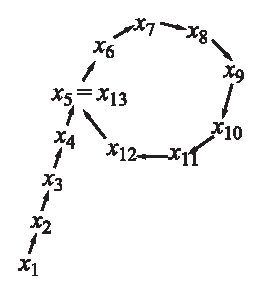
\includegraphics[width=4cm]{ideas/03_13_period/rho.eps}
\begin{center}
\footnotesize
$l=4$, $p=8$.

$x_5=x_{13}$, $x_6=x_{14}$, \dots
\end{center}
\end{wrapfigure}


Пусть у нас есть последовательность, в которой каждый член может принимать одно из $M$ 
значений и является однозначной функцией предыдущего члена. Т.е. $x_1$ задано, а
$$
x_{i+1}=f(x_i),
$$
где $f$ "--- некоторая (известная нам, конечно) функция; причём количество возможных значений 
для каждого члена последовательности есть $M$ (т.е. $f$ "--- это функция, которая в качестве 
своего параметра принимает одно из $M$ допустимых значений и возвращает ещё какое"=то из этих 
же значений). Например, $f(x)=x^2 \bmod M$. Очевидно, что все члены (начиная со второго 
точно) будут целыми числами от 0 до $M-1$.

Тогда очевидно, что у последовательности будет какой"=то период, т.е. начиная с некоторого 
места значения элементов последовательности начнут повторяться. В общем случае возможен также 
и предпериод. Например, если $f(x)=x^2 \bmod 7$ и $x_1=3$, то последовательность будет иметь 
вид 3, 2, 4, 2, 4\dots Видно, что есть период "--- 2, 4; и предпериод "--- 3. В общем случае, 
конечно, и предпериод, и период могут быть разной длины; очевидно только то, что их суммарная 
длина не превосходит $M$ (т.к. первое повторение должно будет произойти максимум на $(M+1)$-м 
числе). Везде в будущем я буду обозначать $l$ "--- минимальная длина предпериода, $p$ "--- 
минимальная длина периода. Замечу, что тогда периодами будут $p$, $2p$, $3p$ и т.д., а 
предпериодами можно считать и $l$, и $l+1$, и $l+2$ и т.д.

Т.е. общая картина будет такая: мы сначала двигается по некоторым числам (по предпериоду), а 
потом выходим на цикл. См. рис.

Часто нам бывает нужно найти длины периода и предпериода нашей последовательности. Например, 
нам на самом деле надо найти член последовательности с очень большим номером $N$. Тогда, найдя
период и предпериод, нам не надо будет вычислять последовательность до $N$-ого члена, а 
достаточно будет знать остаток от деления $N$ на период.

\task|Додумайте тут все оставшиеся детали, т.е., как, зная период, предпериод и 
$N$, найти $N$-й член последовательности. Не забудьте про существование предпериода: а именно, как 
про то, что $N$ может оказаться меньше длины предпериода, так и про то, что период начинается 
не с первого члена.|||||

Обычно нам не надо знать \textit{минимальные} период и предпериод; достаточно знать хоть 
какие"=нибудь (но не слишком длинные). Например, если в вышеприведённом примере мы сочтём, что 
у нас период есть 4 2 4 2, а предпериод "--- 3 2 4 2, то это обычно не страшно (например, в 
задаче нахождения $N$-ого члена последовательности это очевидно не страшно). Мы сосредоточимся 
именно на задаче поиска \textit{каких"=нибудь} периода и предпериода; в конце я ещё скажу на эту тему.

Замечу ещё один момент: пусть вы можете обратить функцию $f$, т.е. выразить $x_i$ через 
$x_{i+1}$ следующим образом: $x_i=f'(x_{i+1})$ с некоторой (новой) функцией $f'$, или, что на самом 
деле то же самое, что для каждого значения $x$ 
существует единственный его "<прообраз"> $x'$ такой, что $f(x')=x$. Тогда это обозначает, что 
по последовательности вы можете двигаться в обе стороны (т.е. по данному элементу находить как 
следующий, там и предыдущий), и это значит, что у неё нет предпериода. Действительно, рассмотрим 
самое первое число, входящее в периодическую часть. Тогда у него есть два 
предшественника: последнее число предпериода и последнее число периода (т.к. после последнего 
числа периода опять идёт первое число периода). Эти два числа различны (иначе наше число не 
было бы самым первым числом периода), что противоречит тому, что по числу однозначно 
определяется его предшественник. То же самое можно сказать по"=другому: начнём с какого"=то 
числа в периоде и будем двигаться назад. Т.к. мы все время можем однозначно определять 
предыдущее число, то ясно, что и двигаясь назад, мы по этому периоду будем мотаться до 
бесконечности и никогда ни в какой предпериод не вывалимся (равно как двигаясь вперёд, мы 
никогда не вывалимся из периода). То же самое: это обозначает, что на рисунке, изображающем 
нашу последовательность (как рис. выше) мы можем обратить стрелки, и из каждого числа тогда 
будет выходить не более одной стрелки. Картинка с предпериодом очевидно этому не 
удовлетворяет.

Поэтому в таком случае вы можете искать период очень просто: просто вычислять один за другим 
элементы последовательности и смотреть, когда повторится \textit{первый} элемент. А повториться он 
обязан, т.к. вы с самого начала находитесь в периоде.

Но далее мы рассмотрим более общий случай, т.е. когда не очевидно, что предпериод отсутствует. 
Как найти какой"=нибудь период и предпериод? Можно поступить по"=тупому, просто запоминая в 
каком"=нибудь массиве, какие элементы уже встречались, и на очередном элементе проверять, не 
встречался ли он раньше. Или проще: завести массив размера $M$ и в нем в соответствующих 
элементах помечать, какие члены последовательности уже встретились.

Но это требует или памяти $O(M)$ (если на каждый элемент заводить свою ячейку массива), или 
памяти $O(l+p)$, но долгого времени, если на каждом шагу искать среди уже встреченных 
элементов наш. Мы же будем строить алгоритмы поиска периода, требующие $O(1)$ памяти и 
$O(l+p)$ времени. Я знаю два способа, которые и изложу ниже.

\textbf{Первый способ: Указатели с разными скоростями.} Заведём два указателя на элементы нашей 
последовательности и будем ими двигаться по ней. (Что я тут имею ввиду под указателями? 
Конечно, не \texttt{pointer} и т.п., а просто переменную, в которой будем хранить значение 
очередного элемента массива.) При этом за один шаг будем сдвигать первый указатель на одну 
позицию, а второй "--- на две:

\pagebreak[3]
\begin{codesampleo}\begin{verbatim}
a:=x1;
b:=x1;
i:=0;
repeat
  a:=f(a);
  b:=f(b);
  b:=f(b);
  inc(i);
until a=b;
\end{verbatim}
\end{codesampleo}

Как это работает? За один шаг расстояние между элементами $a$ и $b$ увеличивается на единицу. 
Как только выполнятся сразу два условия: элемент $a$ вылезет за предпериод (т.е. попадёт в 
период; элемент $b$ идёт впереди элемента $a$, поэтому к этому моменту $b$ уже точно будет в 
периодической части) и расстояние между $a$ и $b$ станет кратным периоду $p$, то тут же 
условие выхода из цикла выполнится и будет найдены период и предпериод: в качестве длины и того, 
и того можно взять $i$: оно всегда равно расстоянию между $a$ и $b$ и равно количеству 
элементов от начала последовательности до $a$.

Если вам до сих пор не понятно, как так получилось, что, если условие 
выполнилось, то в качестве длин периода и предпериода можно взять $i$, то продумайте это ещё 
раз. Можете посмотреть на примерах. Не забудьте, что мы ищем какой"=нибудь предпериод, а не 
кратчайший.

Осталось только понять, что это работает за $O(l+p)$. А это очевидно. За время $O(l)$ элемент 
$a$ доползёт до периодической части (пройдя весь предпериод), а далее не более чем за $O(p)$ 
шагов расстояние между $a$ и $b$ доползёт до числа, кратного $p$. Действительно, за один шаг оно 
увеличивается на единицу, поэтому ползти до числа, кратного $p$, оно будет типа $p-r$ шагов, 
где $r$ есть остаток от деления на $p$ расстояния между ними в момент выхода $a$ в период. 
Значения, кратного $p$ оно не проскочит, т.к. за один шаг увеличивается на единицу.
Значит, действительно это работает за $O(l+p)$.

\task|На первый взгляд может показаться, что надо бы делать проверку $a=b$ два 
раза за цикл: после каждого увеличения $b$:
\begin{codesampleo}\begin{verbatim}
...
  a:=f(a);
  b:=f(a);
  if a=b then break;
  b:=f(a);
...
\end{verbatim}
\end{codesampleo}
типа того (т.е. и соответственно исправить подсчёт длин периода и предпериода), чтобы не получилось 
так, что $b$ "<перескочит"> через $a$. Поймите, почему этого можно не делать.|
||||

\textbf{Способ 2: $\rho$-эвристика.} На самом деле $\rho$"=эвристика "--- это весьма интересный 
алгоритм поиска делителей у больших чисел, использующий поиск зацикливания в 
последовательности и изложенный в том числе в Кормене. Но (по крайней мере в версии алгоритма, 
изложенной в Кормене) там используется другая идея поиска зацикливания в последовательности, 
которую я тут и изложу (а саму $\rho$"=эвристику излагать тут не буду, она далеко не так 
интересна :) ). Кстати, название $\rho$"=эвристики основано на схожести картинки, приведённой 
выше (т.е. картинки зацикливания последовательности) с греческой буквой $\rho$.

Идея такая: возьмём все элементы последовательности, номера которых являются степенями двойки 
(т.е. $a_1$, $a_2$, $a_4$, $a_8$) и (мысленно) разобьём всю последовательность на кусочки, начинающиеся с 
этих элементов:
$$
a_1 | a_2 a_3 | a_4 a_5 a_6 a_7 | a_8 a_9 a_{10} a_{11} a_{12} a_{13} a_{14} a_{15} | 
a_{16} a_{17} \dots a_{30} a_{31} | a_{32} \dots
$$

Будем просматривать кусочки с первого и дальше, и в каждом сравнивать все элементы с первым 
элементом последовательности (точнее, все, кроме первого элемента кусочка; в частности, в первом кусочке нам нечего будет 
делать). Точнее, будем просто двигаться по последовательности, контролируя, в каком кусочке мы 
находимся и сравнивая текущий элемент с первым элементом этого кусочка.

Как только найдём совпадение очередного элемента с первым элементом кусочка, очевидно, что мы 
найдём период (а если подумать, то ясно, что найдётся \textit{кратчайший} период). Тогда 
предпериод можно взять равным расстоянию от начала последовательности до начала текущего 
кусочка.

\task|Попробуйте написать этот код сами. Я его приведу ниже, но постарайтесь 
как"=нибудь написать его сами, прежде чем читать дальше.|||||

За какое время будет найден период? Ясно, что, чтобы нашёлся период, необходимо выполнение 
двух условий: во"=первых, надо, чтобы начала текущего кусочка вылезло за предпериод, 
во"=вторых, надо, чтобы длина кусочка стала не меньше, чем $l$. Первое произойдёт за $O(p)$, 
второе за $O(l)$, Поэтому это работает за $O(l+p)$. (Действительно, когда 
длина периода превзойдёт $l$? Когда длина $2^k$ очередного кусочка превзойдёт $l$. Но тогда 
$2^{k-1}<l$, значит, $2^k<2l$, т.е. $2^k=O(l)$, и аналогично $2^{k+1}=O(l)$ и т.п. Если 
немного подумать, то из таких соображений все следует.)


\pagebreak[3]

\vbox{Итак, обещанный код (как я бы его написал; конечно, можно его и по"=другому писать). Только 
надеюсь, что вы сами сначала подумали над ним. 

\begin{codesampleo}\begin{verbatim}
a:=x1;
k:=1;
i:=1;
while true do begin
      if i=k then begin
         a0:=a;
         k:=k+k;
      end else if a=a0 then
          break;
      inc(i);
      a:=f(a);
end;
\end{verbatim}\end{codesampleo}}

Что я тут делаю? $a$ "--- текущий элемент, $a0$ "--- первый элемент текущего кусочка, $k$ "--- 
номер начала следующего кусочка, $i$ "--- номер текущего элемента. Я думаю, что в остальном 
код понятен, если над ним немного подумать.

Конец $\rho$"=эвристики.

Итак, мы умеем искать период и предпериод, причём даже двумя способами. Теперь ещё пара финальных 
замечаний. Во"=первых, если мы нашли \textit{какие"=нибудь} период и предпериод, то можно найти 
и \textit{минимальные}. Действительно, для начала мы сможем найти минимальный период. Очень просто: 
начав с любого места внутри периода, будем идти до тех пор, пока не встретится то число, с которого 
мы начали. Очевидно, что таким образом мы найдём минимальный период $p$. Далее, для нахождения 
минимального предпериода, будем двигаться параллельно двумя указателями, расстояние между которыми
будет ровно $p$. Т.е. сравним первый и $(p+1)$-ый элементы последовательности. Если они уже равны,
то предпериода, очевидно, нет. Иначе сдвинемся на единицу: сравним 2-ой и $(p+2)$ элементы, и т.д.,
до тех пор, пока не  элементы не совпадут. Когда они совпадут, это будет обозначать, что оба указателя 
вышли из предпериода, причём первый (тот, что указывает на м\'{е}ньший по номеру элемент) вышел из
предпериода только что. Таким образом, мы найдём \textit{минимальный} предпериод. Напоследок ещё раз
замечу, что искать минимальные период и предпериод надо далеко не всегда; в большинстве случаев
может быть достаточно \textit{какого"=нибудь} периода и предпериода.

Напоследок в качестве примера скажу о поиске периода в последовательности остатков чисел Фибоначчи
по данному модулю. А именно, определим $F_0=0$, $F_1=1$, $F_{i+1}=(F_i+F_{i-1}) \bmod M$. Если у 
так определённой последовательности $F$ период? Конечно, есть. Действительно, здесь очередной элемент
определяется \textit{парой} предыдущих, поэтому как только повторится пара, так начнётся период, но
его длину можно оценить сверху только числом $M^2$ (а не $M$, как раньше). (Хотя экспериментально 
оказывается, что для большого количества модулей длина периода сравнима с $M$.)

\note{Более формально можно определить $G_i=(F_i,F_{i+1})$, т.е. как пару из двух последовательных
элементов последовательности. Теперь каждый элемент $G_i$ зависит только от предыдущего, но возможных значений 
элементов стало $M^2$, а не $M$, как раньше.}

Кроме того, заметим, что по этой последовательности мы можем ходить в обе стороны: 
$F_{i-1}\hm=(F_{i+1}-F_i) \bmod M$, поэтому предпериода нет и мы с самого начала находимся в периоде.
Поэтому можно искать период, просто смотря, когда повторятся два числа 0 и 1 подряд.


\lheader{О названиях переменных, отступах и т.д.} 
На самом деле это отдельный сложный вопрос, и большинство в этой теме "--- это вопрос привычки и вкуса. Поэтому не смотрите на это как на обязательные требования, а просто как на какие-то идеи "--- вдруг что полезное для себя узнаете.

Текст написан сначала Оксаной Побуринной (О.П.), потом потом подредактирован мною (П.К.) Большие примечания я писал в скобках, 
но и делал мелкие правки без указания, что это я поправил. Если в других частях я мог 
редактировать текст так, чтобы не приходилось явно писать, где что я добавил, то тут не так, 
поскольку очень многое тут есть вопрос вкуса. 

У каждого человека свой стиль написания программы, свои названия переменных, отступы и т.д. Но, во"=первых, 
нужно, чтобы этот стиль почти не менялся от программы к программе, а во"=вторых, есть неписаные общепринятые 
правила, которых лучше придерживаться. 

\textbf{1.} По поводу названий переменных.

 Во"=первых, полезно привыкнуть в разных программах одно и 
то же называть одними и теми же 
именами. Т.е. если вы привыкли, что $i$, $j$, $k$ "--- это переменные для циклов, $res$ или $ans$ "--- это ответ на задачу,
$cur$, $t$ "--- это некое текущее значение, то по возможности так везде и пишите. Это вам поможет, 
чтобы 1. не думать при написании новой программы, как какую переменную назвать; 2. когда вы глядите на 
программу, вам будет намного проще вспомнить, что какая переменная обозначает.

Во"=вторых, называйте и используйте переменные так, чтобы вам в них не запутаться. Если массивов 
много, не надо называть их $a$, $b$, $c$, $d$, $e$ и $f$. Не  
поленитесь и напишите $cost$, $color$, $was$ и т.д. Конечно, придумывать длинные названия тоже не 
надо, надо почувствовать баланс. Если у вас всего один массив, то напишите $a$ и не беспокойтесь. 
Если два, то не нужно придумывать $IsVertexVisited$ или $VertexLastVisitedTime$, если хватит просто 
$vis$ и $ltime$. Если у вас огромное множество переменных, то, конечно, никуда от фраз вида
\begin{codesampleo}\begin{verbatim}
if (Client[i].status=_free)and(not IsPinging(Client[i].sock)) then begin
или
pALLshutDownAnswer=^tALLshutDownAnswer;
\end{verbatim}
\end{codesampleo}
\noindent не денешься. Но это в больших приложениях, в олимпиадных задачах такого, как правило, не бывает. (полабзаца 
добавлены мною "--- П.К.)

Если у вас все"=таки 4 массива $a$, $b$, $c$, $d$, 
и вы очень хорошо помните, что $n$ "--- размер массива $a$, $m$ "--- размер $b$, $k$ "--- размер 
$c$ и $l$ "--- размер $d$, то пожалуйста, пишите. Только ещё раз подумайте, действительно ли вы так 
хорошо все помните. А лучше как минимум вместо $n$, $m$, $k$ и $l$ написать $na$, $nb$, $nc$ и $nd$ (хотя мне 
это тоже не очень нравится) (\textsl{Да, мне тоже. Потому что нечего называть массивы $a$ \dots{} 
$d$. Назовите массивы по их смыслам "--- хотя бы $w$ если это вес, $name$ если это имя и т.п. "--- 
и тогда пишите хотя бы $nw$, $nname$ и т.п.. Хотя все равно нечасто бывают массивы разной длины в одной программе. "--- 
П.К.})

  Ещё полезно завести себе переменную для обмена "--- такую, которая вряд ли понадобится где-нибудь ещё 
(я лично всегда пишу $ex$ и не думаю, какие из переменных $a$, $b$, $c$, $aa$, $ii$, $jj$, $s$, 
$p$, $q$, $w$ мне не жалко для строчки $ex:=a[i]; a[i]:=a[j]; a[j]:=ex;$ "--- \textsl{А я редко 
пишу обмен где-нибудь, кроме как внутри процедур сортировки, в этих процедурах не так много 
переменных, но все равно завожу специальную $t$ "--- П.К.})
Если в коде много обменов разных типов, то можно и так сделать: вместо \texttt{var s:array [1..100] 
of string;} написать
\begin{codesampleo}\begin{verbatim}
var s:array [0..100] of string;
...
s[0]:=s[i]; s[i]:=s[j]; s[j]:=s[0];
\end{verbatim}
\end{codesampleo}
Т.е. завести дополнительный элемент в массиве и использовать его для обмена. Это гораздо приятнее, чем заводить 
5 новых переменных ради одной"=единственной строчки в коде. \textsl{(Вообще, не жадничайте и не используйте одну и туже переменную в существенно разных целях "--- если у вас нет проблем с памятью, конечно. Если вам нужна временная переменная в отдельном куске программы, не думайте, какая из переменных $i$, $j$ и т.д. у вас не занята тут, а выделите новую переменную. "--- П.К.)}

Также не помешает использовать одни и те же имена для массивов в алгоритмах на графах. В частности, для поисков в глубину и 
ширину "--- хранить, были мы в вершине или нет: например, логические массивы $vis[i]$, 
$visited[i]$, $was[i]$ и т.п. Тут тоже есть проблема "--- часто нужно больше, чем 2 значения был/не 
был: например, в поиске в глубину и ориентированном графе или в поиске в ширину, если нам нужно 
помнить, за сколько шагов мы дошли до вершины и т.п. Тут можно завести массив $c$ (если он больше нигде не 
нужен), $col$ или $color$ для поиска в глубину, массив $d$, $dist$ расстояний для поиска в ширину 
(\textsl{Я не люблю логические массивы: слова true и false больно уж длинные "--- и потому даже в 
случае, когда значений надо всего два, использую массив целых чисел. И пишу в условии 
\texttt{if was[i]<>0}. "--- П.К.})

  Ещё придумайте себе какое-нибудь имя для бесконечности и тоже пишите его одинаково: $INF$, $inf$, $infinity$. 
(\textsl{Ну, конечно, если надо для неё особое имя. Например, в качестве вещественной бесконечности 
я обычно использую $1e20$, и не морочусь с заведением константы для него. Не очень правильно (а 
вдруг придётся её изменять), но эффективно. "--- П.К.})

  Ну и ещё немного. Если раньше написать процедуры nod, nok и poisk было нормально, то сейчас так не модно :) 
Обычно все-таки пишут по-английски, а не транслитом.

Ещё замечание от меня "--- П.К. Если замечаете, что часто перепутываете, как назвать ту или иную 
переменную, выберите один вариант и возьмите в привычку всегда его придерживаться. Два примера: первое: как 
называть массив, например, имён: name или names? Хорошо звучит \texttt{var names:array... of string}: <<\textit{имена "--- 
массив строк}>>. Но потом \texttt{names[i]:=} звучит коряво: <<\textit{имена $i$-ое присвоить}>>. Поэтому 
я для себя решил, что всегда в таких случаях пишу без конечного $s$. Ещё пример: как назвать 
наибольшую координату: $maxx$ или $xmax$? Я так и не решил для себя, а зря. Неприятно бывает, когда 
написал программу и первый раз компилишь её, обнаружить, что в половине мест написал $maxx$, а в половине 
$xmax$\dots

\textbf{2.} Про отступы. Стиль, конечно, у каждого свой, но писать без отступов точно не надо. Это крайне затрудняет чтение 
кода и поиск ошибок. На сколько делать отступ "--- решать вам. Но имхо лучше делать постоянный, например, всегда 1, 
всегда 2 и т.д., а табуляция в паскале таким постоянством не отличается. (\textsl{А мне наоборот 
паскалевский стиль отступов нравится больше "--- П.К.})
Отступ размера 1, мне кажется, маловат: пусть у нас много вложенных циклов
\begin{codesampleo}\begin{verbatim}
for i:=1 to n do begin
 for j:=1 to m do begin
  for ... begin
   //тут много строк кода
  end;
  //тут много строк кода
 end;
 //тут много строк кода
end;    
\end{verbatim}
\end{codesampleo}
Когда begin и end далеко друг от друга, то очень плохо видно, какой end какому begin соответствует. (В принципе, 
это же иногда верно для отступа 2, но в гораздо меньшей степени. Я обычно делаю отступ 2, и меня вполне 
устраивает). Имхо, нормальные отступы "--- 2 или 3. 4 уже много "--- 3 вложенных цикла сильно сдвигают код вправо, 
что опять же неудобно (особенно если в борланде писать, а не в фаре "--- в фаре"=то терпимо ещё более"=менее). 
Опять же надо сказать, что размер отступа зависит от языка программирования. (Например если писать на java 
где-нибудь на работе, когда нельзя переменные называть $a$, $b$, $c$, а нужно писать так, чтобы было понятно, что они 
обозначают, то на фоне функций типа \texttt{Database.Fields.NumberOfDocuments.toString} отступ на 2 символа вообще 
незаметен :) )

  Опять же непонятно, как и где именно делать отступ. Вот примеры:
  
\begin{codesample}\begin{verbatim}
for i:=1 to n do 
begin
  //чего-нибудь
  //
end;

for i:=1 to n do 
  begin
      //чего-нибудь
      //
      end;

for i:=1 to n do 
  begin
      //чего-нибудь
end; (но это вроде совсем изврат:) так писать не стоит)
(собственно, предыдущее тоже изврат имхо --- П.К.)

for i:=1 to n do begin
  //чего-нибудь
end; (это как пишу я-О.П. и я-П.К. :) :)
\end{verbatim}
\end{codesample}

Как последний вариант, тоже писать нехорошо (\textsl{а имхо самый нормальный способ "--- П.К.}), но просто мне 
не нравится писать begin в отдельной строчке "--- когда много циклов, это сильно удлиняет прогу, и 
на экран влезает гораздо меньше.

\textbf{3.} Кстати, как правильно где-то было сказано, \textit{однотипность} отступов, имён и т.д., намного важнее чем сами отступы и т.д. Т.е. если вы редактируете чужую программу, и в ней отступы/пробелы сделаны не так, как вам нравится, то лучше оставить так, как там сделано, и свой код писать в соответствии с теми отступами. И, конечно, если вы пишите свою программу, то тоже стоит все делать однотипно.
